\chapter{Сацыяльнае атачэньне}

\section{Сацыяльны мозг}

Я дапамагаю людзям стаць здаравейшымі, але й яны, у~сваю чаргу, вельмі дапамагаюць мне. Камунікацыя з~разумнымі, моцнымі, крэатыўнымі, упэўненымі людзьмі~--- гэта адна з~самых прыемных характарыстык маёй працы. Ня будзе перабольшаньнем, калі я скажу, што яны мяне натхнялі і падбадзёрвалі ў~важных рашэньнях і справах. Людзі вакол нас заўважна ўплываюць на тое, што мы робім, і тое, як мы сябе адчуваем.

\subsection*{Скажы мне, хто твой сябар, і я скажу, хто ты}

Калі вы камунікуеце з~разумнымі, ветлівымі людзьмі, якія сочаць за сваім здароўем, маўленьнем і вонкавым выглядам, маюць мэты ў~жыцьці ды імкнуцца іх дасягнуць, ня маюць шкодных звычак, добра зарабляюць і бескарысьліва дапамагаюць адно аднаму ў~дасягненьні мэтаў, шчыльна камунікуюць, бавяць час і сябруюць, то з~высокай ступеньню імавернасьці вы будзеце такім жа. Чым больш вы камунікуеце, тым больш задавальненьня атрымліваеце і тым больш вам хочацца гэта рабіць.

А калі вам цяжка знаходзіць агульную мову зь іншымі людзьмі, вы падазроныя, зь цяжкасьцю разумееце іншых і чакаеце ад іх ці то любові, ці то прызнаньня вашых паслуг, калі вашы сябры, знаёмыя і калегі ня сочаць за здароўем, выпіваюць або кураць, безыніцыятыўныя, не разьвіваюцца, кепска выглядаюць і ня сочаць за сабой, то, хутчэй за ўсё, і вы падобныя да свайго асяродзьдзя.

\infobox{Калі вы дрэнна разумееце іншых, ня ўмееце камунікаваць, вам абыякавыя іншыя людзі, то й яны ня будуць імкнуцца падтрымліваць з~вамі сувязі~--- так узьнікае заганнае кола варожасьці і недастатковага разуменьня.}

\emph{Са старажытных часоў людзі жылі невялікімі плямёнамі, дзе ўсе адно аднаго ведалі і ўзаемадзейнічалі. Людзі арганізоўваліся для калектыўнага паляваньня~--- адны высочваюць здабычу, другія гоняць яе, трэція чакаюць у~засадзе,~--- для падтрымкі ў~канфліктах зь іншымі плямёнамі. Уменьне дамаўляцца, разумець адно аднаго і падтрымліваць лягло ў~аснову сучаснай цывілізацыі. У выпадку посьпеху племені перамагаў кожны, а~калі прайгравала племя, то загінуць маглі ўсе.}

Таму ў~нас генэтычна закладзенае імкненьне дапамагаць блізкім людзям, радавацца іх посьпеху. Чым больш пасьпяхова дзейнічае ваша «племя», тым больш посьпеху ў~вас асабіста. А вось дасягнуць вялікіх мэтаў у~адзіночку вельмі складана, таму часта прычынай праблемаў сёньня зьяўляецца ізаляцыя ад неабходных вам людзей, якія маглі б дапамагчы рэалізаваць ваш патэнцыял. 

\textbf{Аптымальнае сацыяльнае атачэньне~--- гэта найлепшае асяродзьдзе для росту, падтрымкі і самарэалізацыі.}

\begin{figure}[htb!]
  \centering
  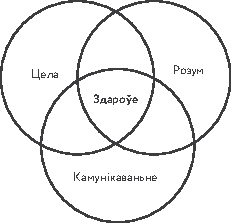
\includegraphics[scale=1.5]{willpower/ch10/1.pdf}
\end{figure}

\subsection*{Сацыяльная ізаляцыя}

Ізаляцыя згубная як для здароўя, так і для кар'еры. ``Выгнаньне з~племені лічылася больш жорсткім пакараньнем, чым кара сьмерцю'',~--- лічылася, што чалавек, ізаляваны ад грамадства, вырачаны на пакуты і гібель. Людзі~--- істоты глыбока сацыяльныя і зьвязаныя з~навакольнымі нашмат мацней, чым мы можам сабе ўявіць.

\emph{Як заўважыў пісьменьнік Оскар Уайльд: «Бываць у~грамадзтве проста нудна. А быць па-за грамадзтвам~--- ужо трагедыя».}

\textbf{Сучасныя ідэі індывідуальнасьці і незалежнасьці} ствараюць ілюзію, што кожны з~нас~--- паўнаўладны гаспадар лёсу, але ў~рэчаіснасьці сацыяльнае атачэньне~--- адзін з~наймагутнейшых рэсурсаў здароўя. Разьвіваючы болей глыбокіх сувязяў, паляпшаючы якасьць камунікацыі, мы мяняем да лепшага як сябе, так і іншых людзей.

Вывучэньне мозгу прыматаў і чалавека паказала, што стылю камунікацыі адпавядае пэўная нэўрахімія мозгу. Напрыклад, у~шымпанзэ высокі ўзровень ацэтылхаліну і нізкі ўзровень дафаміну ў~паласатым целе мозгу, і гэта прыводзіць да таго, што малпы схільныя дзейнічаць, арыентуючыся на ўнутраныя падбухторваньні, ігнаруючы навакольных. У сучасных людзей нэўрахімія мозгу іншая: ужо ў~нашых далёкіх продкаў стала больш дафаміну і сэратаніну і менш ацэтылхаліну. Так мы сталі матываваць сябе тым, што вакол нас, а~не сваімі асабістымі жаданьнямі, навучыліся быць больш уважлівымі да навакольных, улічваць іх інтарэсы, дамаўляцца і, што самае важнае, фармаваць устойлівыя сем'і.

\emph{\textbf{Пакажыце іклы!} Падыдзіце да люстэрка і паглядзіце на свае зубы. Нашыя іклы зусім маленькія~--- і гэта адна з~прыкметаў зьніжэньня агрэсіі да іншых асобінаў.}

Гіпотэза антраполяга Лаўджоя тлумачыць, як разьвіліся \textbf{тры ўнікальныя прыкметы чалавека: кароткія іклы, схаваная авуляцыя і двуногасьць}. Такім чынам, нашыя продкі з~нейкіх прычынаў пачалі практыкаваць сумеснае выкормліваньне дзяцей, бо рэпрадуктыўны посьпех у~прыматаў залежыць ня так ад пладавітасьці, як ад выжывальнасьці дзіцянятаў. Эвалюцыйным посьпехам лічылася манагамная пара і мноства нашчадкаў. Гэта прывяло да разьвіцьця двуногасьці (для таго, каб прыносіць ежу і забясьпечваць самак і дзяцей ежай), зьніжэньня ўнутрыгрупавой агрэсіі за самак і памяншэньня іклоў, якія іх адпужвалі, зьяўленьня схаванай авуляцыі (ніжэйшая імавернасьць прывабнасьці для іншых самцоў). Зьніжэньне ўнутрыгрупавой агрэсіі прывяло да лепшай каапэрацыі і стымулявала разьвіцьцё галаўнога мозгу.

Цалкам магчыма, што менавіта манагамія зрабіла нас людзьмі. Калі самцы перастаюць канкураваць за самак, то ім лягчэй дамаўляцца паміж сабой і каапэравацца для здабычы ежы. Таму зьмена нэўрахіміі нашага мозгу прывяла да мацнейшага кантролю над эмоцыямі, стрымліваньня агрэсіі і ўтварэньня доўгатэрміновых сувязяў~--- у~выглядзе як сем'яў, так і ўстойлівых сяброўскіх стасункаў.

\textbf{Наш мозг зьмяніўся і стаў нашмат больш сацыяльным, мы сталі жыць у~сем'ях і сябраваць сем'ямі.} Усталяваньне шматлікіх сямейных і сяброўскіх сувязяў спрыяла назапашваньню культурных навыкаў і далейшай эвалюцыі і прагрэсу. «Сэкс-бомбы» і «дрэнныя хлопцы»~--- гэта не адаптацыя, а~водгульле старэйшай праграмы паводзінаў.

Актыўнае сацыяльнае жыцьцё ў~племені, актыўныя ўзаемадзеяньні зь людзьмі~--- усё гэта прыводзіла да таго, што сацыяльны статус і лепшае разуменьне адно аднаго стала забясьпечваць большы рэпрадуктыўны посьпех. Пераход ад герархіі да эгалітарызму прывёў да таго, што вырашальнай стала не фізычная сіла, а~інтэлект, уменьне пралічваць учынкі іншых, разумець матывацыю і пачуцьці суродзічаў, мець у~галаве дынамічныя мадэлі іх псыхікі. Чым больш у~нас кантактаў, тым большае разьвіцьцё зонаў мозгу, адказных за памяць і распазнаньне людзей.

\subsection*{Тэорыя сацыяльнага мозгу}

Тэорыя сацыяльнага мозгу лічыць, што менавіта ўзаемадзеяньне з~суродзічамі было і ёсьць рухальнай сілай эвалюцыі. Наш «сацыяльны мозг» уключае многія аддзелы мозгу: лобныя долі, скроневыя, мігдаліну і да т.~п. Разуменьне іншых людзей~--- гэта надзвычай складаны навык, бо трэба адрозьніваць намёкі, падман, разумець інтанацыі, міміку, супастаўляць гэта з~сытуацыяй і асаблівасьцямі чалавека~--- усё гэта патрабуе інтэнсіўнага разьвіцьця мозгу.

\begin{figure}[htb!]
  \centering
  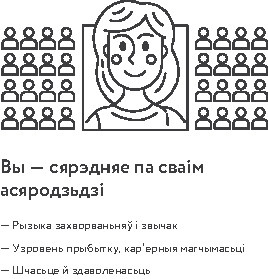
\includegraphics[scale=1.5]{willpower/ch10/2.pdf}
\end{figure}

\infobox{У сярэднім чалавек можа сябраваць, то бок рэгулярна падтрымліваць адносіны, даведвацца і памятаць характарыстыкі 150 чалавек (а некаторыя «прасунутыя карыстальнікі» і больш за 200), што ўдвая больш, чым малпы.}

\emph{Гэта называецца «колькасьць Данбара» і сьведчыць пра абмежаваньне колькасьці пастаянных сацыяльных сувязяў. Лік 150 увесь час прайграецца ў~чалавечай гісторыі: сярэдні памер вёскі, колькасьць людзей у~племені, памер ваеннага атрада, колькасьць актыўных сяброў у~сацсетках і г.~д.}

Сацыябэльнасьць чалавека карэлюе з~памерамі лобных і скроневых доляў чалавека, якія павялічваліся ў~працэсе эвалюцыі.

\emph{Пашкоджаньне асобных частак мозгу, напрыклад лобных доляў, прыводзіць да таго, што людзі хоць і захоўваюць памяць пра сацыяльны сьвет і яго нормы, але робяць моцныя памылкі ва ўспрыманьні эмоцыяў, невэрбалікі, ня могуць разумець іронію ці даваць слушныя маральныя ацэнкі.}

Такім чынам, нашае мысьленьне шчыльна завязанае на сацыяльным асяродзьдзі і ўзаемадзеяньні зь ім. Зьбядненьне колькасьці сувязяў вельмі ўплывае на нашае здароўе~--- як прама, так і ўскосна, праз узровень стрэсу, атрыманьне важных ведаў і да т.~п. Для адэкватнага сацыяльнага ўзаемадзеяньня важныя разьвітыя сацыяльныя навыкі. Многія людзі не атрымліваюць усіх магчымых задавальненьняў ці пераваг ад камунікацыі, бо маюць неадаптыўныя мадэлі паводзінаў, засвоеныя яшчэ зь дзяцінства. 

Важную ролю ў~камунікацыі граюць \textbf{люстраныя нэўроны}, дзякуючы якім мы можам аўтаматычна прайграваць эмацыйныя рэакцыі нашага бліжэйшага атачэньня, менавіта таму так важна заўсёды сачыць, хто знаходзіцца навокал. Атачэньне дае нам мноства сыгналаў, якія ўхваляюць ці крытыкуюць тое, што мы робім і як рэагуем на стымулы, і такім чынам навучае нас. Наш унутраны сацыёмэтар успрымае ўзровень грамадзкае ўхвалы, яго зьмены прыкметна адбіваюцца на нашым самаадчуваньні. На падставе грамадскае ўхвалы мы мадэлюем і свае паводзіны. Таму ад навакольных можа залежаць, возьмемся мы за пэўныя праекты ці не, будзем упартыя ці здадзімся. Люстраныя нэўроны могуць прыносіць нам радасьць, калі людзі вакол усьміхаюцца, але калі вакол нас пахмурныя твары, то й наш настрой будзе зьніжацца.

\textbf{Можна і трэба вучыцца камунікацыі.} Многія людзі ўспрымаюць таварыскасьць як нейкую спрадвечную прыроджаную характарыстыку чалавека. Нехта сьцьвярджае, што ён~--- інтравэрт, і яму не наканавана камунікаваць ушчыльную. Іншыя баяцца падацца дурнаватымі ці нягеглымі, стаць аб'ектам насьмешак. Насамрэч кожны з~нас, нават глыбокі інтравэрт, звышсацыяльны. Цяга да камунікацыі, уменьне разумець іншых закладзеныя ў~нашых генах, трэба толькі рэалізаваць гэты навык, навучыцца карыстацца інструмэнтам. Чым больш мы будзем разумець іншых людзей, вывучаць іх, тым цікавейшымі яны нам пададуцца. Чым больш цікавасьці мы да іх адчуваем, тым больш нязмушанай і яркай будзе камунікацыя. Адпаведна, чым больш задавальненьня мы атрымаем, тым больш актыўна будзем знаёміцца і ўзаемадзейнічаць з~навакольнымі.

Нам патрэбныя іншыя людзі, каб пераадолець сваю ізаляцыю і адзіноту. Але зьявіцца яны могуць, калі мы дапаможам ім у~гэтым. Ня трэба рабіць ідэю ``адзіноты'' рамантычнай і цудоўнай, у~ёй няма нічога карыснага, яна небясьпечная для здароўя. Пераадолейце свае перадузятасьці і чаканьні ад іншых людзей, ідзіце ім насустрач. Дапамажыце іншым пазбавіцца ад адзіноты і забабонаў у~дачыненьні да камунікацыі, гэта ўзбагаціць кожнага з~вас.

\emph{У дзяцінстве я мала камунікаваў з~аднагодкамі, аддаваў перавагу ўсё рабіць і вывучаць самому. Пасьля заканчэньня мэдыцынскага ўнівэрсытэта пайшоў на спэцыялізацыю анэстэзіёляг-рэаніматоляг адно з~тае прычыны, што лекары гэтай спэцыяльнасьці менш за ўсё маюць зносіны з~пацыентамі (а таксама мне падабалася рэаніматалёгія і прыборы). Але, пачаўшы выкладаць у~мэдыцынскім унівэрсытэце, а~затым у~сваёй школе здароўя, я разьвіў навыкі зносінаў і стаў атрымліваць нашмат больш задавальненьня ад камунікацыі і новых людзей. Зрэшты, мне яшчэ вельмі далёка да «камунікатыўных геніяў».}

\begin{figure}[htb!]
  \centering
  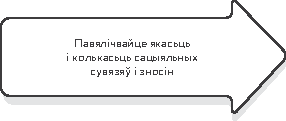
\includegraphics[scale=1.5]{willpower/ch10/3.pdf}
\end{figure}

\subsection*{Інвэстуйце ў~сувязі}

Сацыяльныя адносіны~--- гэта важны рэсурс, у~яго варта сыстэмна інвэставаць, бо добрыя сувязі не ўзьнікаюць самі па сабе. Стывен Кові, аўтар кнігі ``Сем навыкаў высокаэфэктыўных людзей'', апісвае адносіны як стварэньне эмацыйнага банкаўскага рахунку, які вызначае ўзровень даверу ў~адносінах.

\infobox{Калі вы паважліва і сумленна ставіцеся да чалавека на рэгулярнай аснове, ягоны давер да вас расьце.}

Высокі ўзровень даверу робіць магчымым эфэктыўныя камунікацыю, супрацоўніцтва, каапэрацыю.

\textbf{Нават памылкі могуць быць дараваныя пры высокім капітале даверу.} Але калі вы камунікуеце непаважліва, злоўжываеце даверам, не даяце чалавеку выказвацца, ігнаруеце ці раздражняецеся, то ваш эмацыйны рахунак растае. Пры нізкім узроўні даверу да вашых словаў і прапановаў ставяцца насьцярожана і падазрона, што абцяжарвае камунікацыю і разбурае яе. Гэта можа адбывацца як між мужам і жонкай, так і ўнутры кампаніі.

\subsection*{Пытаньні і заданьні}

1. Вы~--- тыповы прадстаўнік вашага атачэньня ці не?

2. Ці падзяляеце вы посьпех вашых сяброў альбо зайздросьціце яму?

3. Наколькі таварыскім вы сябе лічыце? Ці спрабавалі вы разьвіваць гэты навык?


\section{Эпідэмія самоты}

Навукоўцы сур'ёзна занепакоеныя эпідэміяй самоты. Сябры і камунікацыя~--- гэта незаменныя вітаміны для нашага мозгу, бо ўся гісторыя чалавека прайшла ў~цесным кантакце зь іншымі: ад вялікай сям'і да згуртаванай супольнасьці. Самота, нават не ўсьвядомленая, глыбока нефізыялягічная для нашага арганізма, нам эвалюцыйна прызначана быць у~кантакце са сваякамі й суродзічамі. Наш мозг успрымае змушаную адзіноту як сымптом хваробы і рэагуе на яго адпаведна.

Але цяпер грамадства ўсё больш атамізуецца, распадаецца. З аднаго боку, у~нас усё больш магчымасьцяў мяняць сваё атачэньне, вандраваць, быць на сувязі. Адваротны бок мабільнасьці~--- гэта зьніжэньне колькасьці доўгатэрміновых сувязяў і слабоя ўкараненьне людзей. Мы бачым, што ўсё больш людзей пачуваюцца самотнымі: у~заходніх краінах гэтая лічба складае 20--40\,\% дарослага насельніцтва. Сучаснае грамадства часта завуць ``вадкім'' (liquid society), калі сталыя пераезды прыводзяць да таго, што ў~нас менее грамадзкіх сувязяў, мы надаём недастаткова ўвагі адносінам у~адрозьненьне ад традыцыйнай мадэлі вялікай сям'і, дзе пад адным дахам жывуць розныя пакаленьні.

\emph{У Японіі паўмільёна хікікіморы (хікі)~--- людзей, якія імкнуцца да поўнай сацыяльнай ізаляцыі, у~Швэцыі амаль палова гаспадарак~--- гэта самотныя і бязьдзетныя дарослыя людзі, у~Брытаніі больш за 9 мільёнаў самотнікаў і самотніц, у~ЗША больш за 40 мільёнаў людзей старэйшых за 45 гадоў самотныя. Калі ў~1900 годзе толькі 5\,\% людзей лічылі сябе самотнымі, дык цяпер іх ня менш за 25\,\%. Скарачаюцца і спосабы баўленьня часу, мы ўсё меней зьбіраемся разам на мерапрыемствы, радзей гуляем у~гульні або займаемся спортам. Нават у~межах адной сям'і людзі ўсё менш камунікуюць і радзей ядуць за адным сталом.}

Прычынаў багата: гэта і зьмена эканамічных адносінаў, калі зьяўленьне пэнсій зрабіла пэнсіянэраў незалежнымі, і фінансавая незалежнасьць кожнага чалавека, які можа дазволіць сабе забясьпечваць выдаткі на жыцьцё самастойна, і ўзмацненьне дзяржавы. Парадокс: чым больш мы давяраем дзяржаве, тым меншая неабходнасьць зьвяртацца па дапамогу да сяброў. Ва ўсім сьвеце цяпер адбываецца зьніжэньне цікавасьці да грамадскіх аб'яднаньняў, памяншэньне колькасьці добраахвотных асацыяцыяў. Гэтыя працэсы могуць быць даволі небясьпечнымі для дэмакратычных краінаў, бо зьмяншаюць салідарнасьць грамадства.

\textbf{Гарадзкое асяродзьдзе.} Большую частку сваёй эвалюцыі чалавек праводзіў у~атачэньні людзей, якіх ён добра ведаў ці якія былі яго сваякамі, сустрэчы зь незнаёмцамі адбываліся рэдка. Чым больш вакол нас людзей, тым цяжэй нам падтрымліваць зь імі сувязь: сёньня жыхары буйных гарадоў ня ведаюць нават сваіх суседзяў, а~лішак незнаёмцаў павялічвае стрэс ад высокай няпэўнасьці і недахопу кантролю. Парадаксальна, але больш высокая фізычная шчыльнасьць людзей прыводзіць да росту псыхалягічнага адчужэньня.

Пераязджаючы, я заўсёды знаёмлюся з~суседзямі і бяру ўдзел у~грамадзкіх справах. Вядома, часта ў~вялікім горадзе людзі разьяднаныя і іх цяжка арганізаваць, скажам, на тое, каб разьбіць кветнікі на вуліцы ці адрамантаваць пад'езд. Таму часта большую частку затратаў даводзілася браць на сябе асабіста, але ў~працэсе звычайна хто-небудзь далучаўся. Лішак незнаёмых людзей павялічвае стрэс, а~высокая фізычная шчыльнасьць насельніцтва вядзе да росту псыхалягічнага адчужэньня.

\textbf{Высакашчыльнае гарадзкое асяродзьдзе} ня вельмі спрыяльнае для фізычнай актыўнасьці: колькасьць прагулачных сьцежак і бясьпечных грамадскіх месцаў скарачаецца. Яно таксама спрыяе і нездароваму харчаваньню праз мноства крамаў і рэстарацыяў, рэклямы фастфуду, дарагіх якасных прадуктаў. Высокі ўзровень стрэсу павялічвае і вялікую імавернасьць дэпрэсіі ды трывожных разладаў. Сувязь шчыльнасьці насельніцтва і ўзроўню шчасьця неадназначная ў~розных частках сьвету. На індывідуалісцкім Захадзе дзейнічае правіла, што гараджане менш шчасьлівыя: чым большы горад, тым меншы ўзровень шчасьця. Іншыя дасьледаваньні абвяргаюць гэта і гавораць пра большую сувязь шчасьця і даходу: у~Азіі, дзе ёсьць схільнасьць да калектывізму, жыхары буйных гарадоў пачуваюцца шчасьлівейшымі.

Колькасьць злачынстваў у~хмарачосах павялічваецца амаль прапарцыйна іх вышыні. Калі ў~трохпавярховых дамах учыняецца 8,8 злачынстваў на тысячу жыхароў, то ў~шаснаццаціпавярховых~--- да 20,2. Таксама гараджане значна часьцей пакутуюць на разнастайныя парушэньні псыхікі, напрыклад трывожны нэўроз і афэктыўны разлад. Навукова даведзеная сувязь актыўнасьці мігдаліны і шчыльнасьці насельніцтва: чым у~буйнейшым населеным пункце жыве чалавек, тым мацней актывуецца ў~яго мігдаліна ў~адказ на стрэс.

\infobox{Анляйн-камунікацыя наўрад ці заменіць рэальную: у~ёй няма фізычнага кантакту, невэрбальны кантакт~--- слабы, і няма магчымасьці атрымліваць досьвед сумеснага пражываньня падзеяў.}

Чым большы горад, тым больш адзіноты: высокая шчыльнасьць людзей спрыяе адчужанасьці. Тут часта выяўляецца звышасьцярожнасьць, калі людзі не карыстаюцца наяўнай магчымасьцю для камунікацыі, лічачы самоту больш спакойнай. Але гэта наша памылка, калі мы думаем, што самота палепшыць нашае самаадчуваньне. Насамрэч, яна можа адно пагоршыць яго, а~вось камунікацыя~--- дапамагае.

\emph{У буйных гарадах ужо зьявілася паслуга ``сябар на гадзіну'', калі вы можаце купіць увагу іншых людзей.}

Анляйн-камунікацыя ня можа замяніць рэальную, бо практычна 80\,\% успрыманьня~--- гэта невэрбальная інфармацыя (позірк, гэсты і г.~д.) суразмоўцы і агульны для вас кантэкст, які аб'ядноўвае (вы ў~адзін час у~адным месцы і пражываеце разам адзін момант). А вось пры камунікаваньні анляйн вы не атрымліваеце ўсёй інфармацыі пра суразмоўцу, вы ў~розным кантэксьце, мо нават у~розныя моманты часу. Усё гэта вядзе да таго, што мы губляем значную частку таго, што хочам данесьці, і нашмат горш разумеем суразмоўцу. Таму ўзьнікае моцнае скажэньне, якое прыводзіць да неадэкватных высноваў і заключэньняў. А сфармаванае меркаваньне потым ужо цяжка будзе зьмяніць.

\textbf{Камунікацыйны голад.} Само па сабе пачуцьцё самоты не небясьпечнае, гэта біялягічны сыгнал нашага арганізма, як смага ці голад, і задаволіць яго можна камунікацыяй. Каб выжыць, камунікуй зь іншымі~--- так кажа нам інстынкт. Голад можна задаволіць як якаснай ежай, карыснай для здароўя, так і фастфудам, які яго сьцішае, але шкодны ў~пэрспэктыве. Задаволіць пачуцьцё самоты можна і сацсеткамі ці плёткамі, але ў~пэрспэктыве злоўжываньне анляйн-камунікацыяй пагаршае сытуацыю. Можна забіць пачуцьцё адзіноты і заяданьнем, тады фармуецца заганнае кола: я самотны, таму тоўсты, і я тоўсты, таму самотны.

Ясная рэч, ня варта кідацца ў~скрайнасьці і лічыць любую адзіноту шкоднай. У гэтым разьдзеле гаворка ідзе менавіта пра змушаную самоту. Дасьледаваньні паказваюць, што людзі з~больш высокім IQ менш маюць патрэбу ў~сябрах і атрымліваюць задавальненьне ад жыцьця. Па сутнасьці, быць аднаму, жыць аднаму і быць адзінокім~--- гэта розныя рэчы, якія па-рознаму ўплываюць на здароўе.

\begin{figure}[htb!]
  \centering
  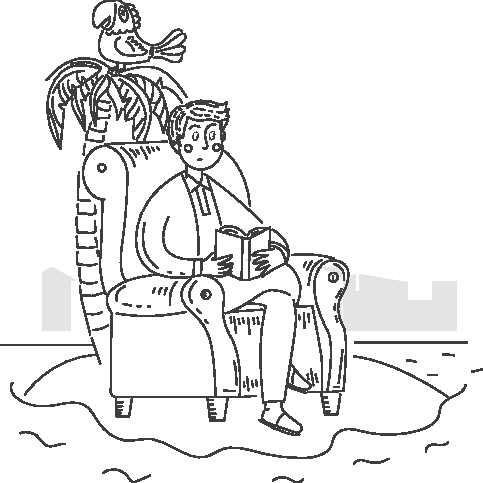
\includegraphics[scale=0.9]{willpower/ch10/4.pdf}
\end{figure}

\subsection*{Пытаньні і заданьні}

1. Ацаніце вашыя сацыяльныя сувязі якасна і колькасна. Ці дастаткова іх вам?

2. Ці любіце вы быць сам-адзін? У якіх сытуацыях быць аднаму прыемна?

3. Што вы робіце, калі адчуваеце самоту?


\section{Сацыяльнае атачэньне і здароўе}

Лепш сто сяброў, чым сто рублёў: сапраўды, а~колькі каштуе сябар? Ацэнкі, праведзеныя ў~ЗША, паказваюць, што калі самотны чалавек заводзіць моцнае сяброўства, то ўзьдзеяньне на ўзровень шчасьця аналягічнае павышэньню гадавога заробку на 60 тысячаў даляраў.

Сяброўства і камунікацыя~--- гэта прафіляктыка і лячэньне шматлікіх захворваньняў. Нават прымаўка ёсьць: чалавек безь сяброў што печ бяз дроў. Адчуваньне сувязі зь іншымі людзьмі~--- гэта глыбінная патрэба чалавека, таму калі ўжо не сяброўства, то актыўны ўдзел у~сацыяльных справах, напрыклад валанцёрства, таксама павышае ўзровень задавальненьня. Адзін з~надзейных спосабаў справіцца з~болем~--- гэта дапамагаць іншым людзям, якім яшчэ горш. А вось сацыяльная ізаляцыя або адрыньваньне, здрада блізкіх выклікаюць боль ня менш рэальны, чым фізычны, і да таго ж ён можа не згасаць з~часам.

Калі дыета і фізычная актыўнасьць могуць да 20--30\,\% зьнізіць рызыку сьмяротнасьці, то сямейная і сяброўская падтрымка зьніжае яе на 45\,\%, а~моцны шлюб~--- на 49\,\%. Вельмі важна і карысна часьцей бываць сярод людзей, якія вас шчыра любяць, людзей, якія даюць вам паверыць у~сябе, людзей, якія чакаюць ад вас посьпеху.

\emph{Навукоўцы ацанілі шкоду змушанай самоты, прыраўняўшы яе да 15 скураным цыгарэтам у~дзень, што перавышае нават небясьпеку атлусьценьня і маларухомага ладу жыцьця. Рызыка раньняй сьмерці сярод людзей, якія адчуваюць адзіноту і пакінутасьць, павялічваецца на 26\,\%, жыцьцё на самоце ў~кватэры ці доме~--- на 32\,\%, сацыяльная ізаляцыя~--- на 29\,\%.}

\infobox{Прыналежнасьць да рэлігійных суполак зьніжае рызыку сьмерці на 20\,\%, што было даведзена на прыкладзе прыхаджанаў цэркваў. Апроч зьніжэньня рызыкі шэрагу захворваньняў, гэта спрыяе ўсталяваньню дадатковых сацыяльных сувязяў.}

У самотных вышэйшая рызыка ішэмічнай хваробы сэрца, гіпэртаніі, інсульту, дэмэнцыі, суіцыдальных спробаў і дэпрэсіі. Адзінота павялічвае рызыкі для здароўя, уплываючы на маркеры здароўя, такія як ліпідны профіль, С-рэактыўны бялок, артэрыяльны ціск і да т.~п. Мэханізмы ў~гэтага розныя: разьвіцьцё дэпрэсіі, зьніжэньне фізычнай актыўнасьці, павелічэньне ўзроўню стрэсу, зьніжэньне ўзроўню падтрымкі, грэбаваньне мэдыцынскім абслугоўваньнем і да т.~п. Калі вы шмат часу праводзіце сярод іншых, то вам важна, як вы выглядаеце, як вы рухаецеся, таму вы сочыце за харчаваньнем і актыўнасьцю. Праз сацыяльную ізаляцыю зьяўляецца жаданьне ``запусьціць сябе'', павышаецца рызыка шкодных звычак, такіх як курэньне і алькагалізм.

\textbf{Маладыя і пажылыя людзі найболей уразьлівыя перад ізаляцыяй.} Разьвітыя сацыяльныя сувязі ў~падлеткаў абараняюць ад атлусьценьня ня горш, чым рухальная актыўнасьць. Чым больш у~чалавека ва ўзросьце значных адносінаў зь іншымі людзьмі, тым лепш працуе мозг і менш рызыка Альцгаймэра. Анкалягічныя пацыенты лепш пераносяць хіміятэрапію, калі ў~іх ёсьць суседзі па палаце. У таварыскіх людзей меншая рызыка дыябэту 2 тыпу, а~ў людзей з~дэфіцытам камунікацыі рызыка дыябэту ўзрастае на 42\,\% у~мужчынаў і на 112\,\% у~жанчынаў. Страта кожнага сябра на 12\,\% павялічвае рызыку дыябэту.

\infobox{Варожасьць і недружалюбнасьць павялічваюць сьмяротнасьць ад сардэчна-сасудзістых захворваньняў незалежна ад іншых фактараў.}

Пры адзіноце мозг пачынае менш актыўна рэагаваць на станоўчыя стымулы і становіцца больш адчувальны да нэгатыўных, што пагаршае стрэсаўстойлівасьць. Самотным людзям трэба болей часу, каб заснуць, яны часьцей прачынаюцца ноччу і менш глыбока сьпяць. Нават невялікая размова зь незнаёмцамі або малазнаёмымі людзьмі зьніжае ўзровень стрэсу; павелічэньне колькасьці нават слабых сацыяльных сувязяў~--- напрыклад, прадавец крамы або сусед па доме,~--- дабратворна ўплывае на стрэсаўстойлівасьць і ўзровень шчасьця. А вось вварожасьць і непрыязь павялічваюць сьмяротнасьць ад сардэчна-сасудзістых захворваньняў незалежна ад іншых чыньнікаў. 

\subsection*{Соцыюм і актыўнае даўгалецьце}

У доўгажыхароў Акінавы ёсьць такія традыцыі, як мааі, юімару, наараі.

\textbf{Актыўнае сацыяльнае жыцьцё (мааі)}~--- гэта супольны лад узаемавыручкі, неад'емная частка іх ладу жыцьця: побач з~акінаўцам заўсёды ёсьць сябры і іх фінансавая і псыхалягічная падтрымка. Нават разуменьне, што ў~выпадку бяды ты ня будзеш самотны, ужо дае антыстрэсавы эфэкт. Мааі~--- гэта сустрэчы аднадумцаў, якія зьбіраюцца для падтрымкі каго-небудзь або для заняцьця агульнай справай. Нават цяпер да 50\,\% акінаўцаў уваходзяць у~мааі, часта адзін чалавек уваходзіць у~некалькі мааі~--- гэта могуць быць школьныя таварышы ці «клюбы па інтарэсах».

\textbf{Юімару (мару~--- кола)~--- гэта праява роўнасьці, а~наараі (праламленьне хлеба)~--- гэта традыцыя прымаць ежу ў~кампаніі блізкіх.} Сумеснае сталаваньне як у~коле сям'і, так і зь сябрамі і калегамі~--- вельмі карысная ідэя, старайцеся радзей есьці ў~адзіноце. Для даўгалецьця важна і тое, што пажылых паважаюць, яны захоўваюць права прыняцьця рашэньняў, зьяўляюцца апорай сям'і і аўтарытэтам.

\emph{На жаль, у~многіх заходніх краінах пажылыя людзі альбо аказваюцца ў~ізаляцыі, альбо трапляюць у~дамы састарэлых, дзе іх самастойнасьць абмяжоўваецца, што вельмі шкодна для здароўя і даўгалецьця.}

Цікавым прыкладам зьяўляецца і эфэкт Разэта. Гэта горад, заснаваны італьянскімі мігрантамі ў~Пэнсільваніі. Разэта прыцягнуў увагу дасьледнікаў нізкім узроўнем сардэчна-сасудзістых захворваньняў~--- удвая меншым, чым у~цэлым па ЗША. Дасьледаваньні паказалі, што \textbf{асаблівых адрозьненьняў у~ладзе жыцьця ў~жыхароў няма, за выключэньнем дзіўнай арганізацыі сацыяльнага жыцьця}: 22 грамадскія арганізацыі ў~мястэчку на 2000 чалавек, дух раўнапраўя і роўнасьці, вялікія сем'і з~традыцыямі павагі старэйшых, клопат жыхароў адно пра аднаго і адчуваньне згуртаваньня і адзінства.

\subsection*{Узровень даходу}

Ваш сярэдні даход роўны сярэдняму арыфмэтычнаму даходу найбольш значных для вас людзей у~вашым асяродзьдзі. Калі вы ў~сярэдняй траціне вашых сяброў па даходзе, то ваша імавернасьць больш зарабляць у~бліжэйшыя гады высокая, а~калі вы ў~верхняй траціне~--- то шанцы падняць свой даход памяншаюцца ў~шмат разоў. Забясьпечаныя сябры аўтаматычна стымулююць вас зарабляць больш, пры гэтым лепей каб яны былі багацейшымі за вас, скажам, ня ў~тысячу, а~ў два разы.

\subsection*{Пытаньні і заданьні}

1. Як уплывае на вашае здароўе ізаляцыя?

2. Ці камфортна вам сярод тых людзей, якіх вы ведаеце?

3. Ці дапамагае камунікацыя лепшаму самаадчуваньню пры стрэсе або хваробе?


\section{Сацыяльныя сувязі}

У працэсе эвалюцыі ў~нашых продкаў паступова павялічваліся магчымасьці мозгу, каб запамінаць і апрацоўваць псыхалягічныя мадэлі стану розных людзей. Як мы ўжо казалі, сярэдняя колькасьць сувязяў~--- 150, ад 100 да 230 чалавек. Калі колькасьць расьце, мозгу цяжэй памятаць кожнага і выбудоўваць з~ім адносіны. Бо для падтрыманьня ўсіх гэтых сувязей актуальнымі патрабуецца час і намаганьні. Калі ў~вас узьнікаюць новыя кантакты, старыя паступова зьнікаюць.

\emph{Памер сярэдняга племені ў~паселішчах каменнага веку не перавышаў 200 чалавек; калі людзей ставала болей, племя дзялілася.Сярод супляменьнікаў усе адно аднаго ведалі, памяталі і стваралі стабільныя адносіны.}

Ёсьць і больш шчыльныя групы: падзелім 150 на 3 і атрымаем 50~--- гэта памер групы аднадумцаў, калег. А група з~15 чалавек~--- гэта тыя людзі, падзеі ў~жыцьці якіх эмацыйна ўплываюць на нас і цікавыя нам. Падзелім яшчэ на 3~--- атрымаем 5. Пяць чалавек~--- гэта самыя блізкія людзі, зь якімі мы можам падзяліць свае патаемныя жаданьні і страхі. Або можна ўмоўна вылучыць узровень сям'і, затым блізкіх сяброў, на якіх можна разьлічваць, затым ``племя'' ці ``вёска'' (агульныя інтарэсы) і ўзровень ``слабых сувязяў'', уключаючы інтэрнэт-сяброў.

\textbf{Зрабіце простае практыкаваньне}: выпішыце ўсіх людзей, з~кім вы камунікуеце і пачуваецеся камфортна. Колькі атрымалася? Цяпер разьбіце іх па групах~--- блізкае кола, сярэдняе, далёкае~--- ці ўсе ў~вас ёсьць? Памятайце, што месца ў~нашым мозгу могуць займаць ня толькі рэальныя, але і выдуманыя або віртуальныя пэрсанажы, мэдыяпэрсоны. Вы можаце сачыць за сваім кумірам, калі вучыцеся ў~яго нечаму карыснаму.

\emph{Калі мозгу бракуе камунікацыі, ён гатовы занурыцца ў~бульварныя плёткі. Але ці сапраўды вам трэба ведаць розныя фэйкавыя «зорныя» навіны?! Камунікацыя з~рэальнымі людзьмі нашмат карысьнейшая для здароўя.}

\infobox{Кожная сувязь характарызуецца сваёй «сілай»: чым больш працяглыя стасункі, чым вышэйшая эмацыйная блізкасьць, давер і чым часьцей мы робім адно аднаму ўзаемныя паслугі, тым мацнейшая сувязь. Але вялікае значэньне маюць і ``слабыя'' сувязі.}

\textbf{Слабыя сувязі}~--- гэта людзі, зь якімі мы сустракаемся, але не знаёмыя блізка: калегі, суседзі, прадаўцы, былыя аднаклясьнікі і да т.~п. Яны не зьяўляюцца нашымі сябрамі і адносяцца да іншых клястараў, і, такім парадкам, могуць даць нам доступ да новай інфармацыі, ідэй, знаёмстваў, магчымасьцяў і да таго ж прывесьці да пашырэньня нашага ўплыву. Гэтыя сувязі могуць быць значна больш разнастайнымі, плюралістычнымі, і мы можам падтрымліваць тысячы такіх «слабых» сацыяльных сувязяў.

\begin{figure}[htb!]
  \centering
  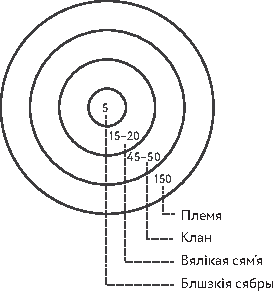
\includegraphics[scale=1.5]{willpower/ch10/5.pdf}
\end{figure}

\subsection*{Як павялічыць свой сацыяльны капітал}

Вядома, ня варта хадзіць і высільвацца, каб з~кім-небудзь пасябраваць, калі ўжо гэта карысна для здароўя. Аднавіць старую сувязь лягчэй, чым выбудаваць новую: складзіце сьпіс добрых знаёмых, якія выпалі з~поля ўвагі, і аднавіце гэтыя адносіны. Знаёміцца~--- гэта навык, які трэніруецца гэтак жа, як іншыя навыкі. Пра гэта напісаныя кнігі, ёсьць курсы камунікацыі і прамоўніцкага майстэрства. Калі вам замінаюць псыхалягічныя праблемы, то дапаможа псыхатэрапія. Навык прыходзіць і ўмацоўваецца толькі з~практыкай, таму трэніруйцеся ўсюды, дзе будзе дарэчы знаёміцца і ўступаць у~кантакт.

\begin{figure*}[htb!]
  \centering
  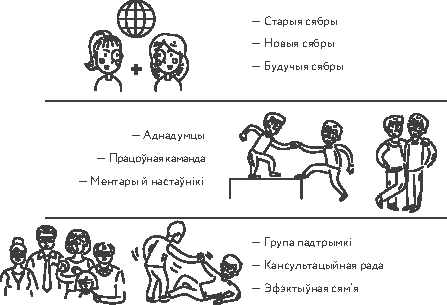
\includegraphics[scale=1.5]{willpower/ch10/6.pdf}
\end{figure*}

\emph{``Мяне клічуць Андрэй, я пішу кнігу, яна дапаможа вам стаць здаравейшымі і прыгажэйшымі'',~--- калі вы назваліся, вам прасьцей выказвацца і заводзіць знаёмствы. У гутарцы будзьце прыязныя, дапамагайце людзям і шчыра цікаўцеся імі, тады вы будзеце ненавязьлівыя і самі атрымаеце задавальненьне і прыемны посмак. Спытайце сябе, чаму вы можаце навучыцца ў~гэтага чалавека? Вучыцеся і самі быць цікавымі і крэатыўнымі, разумець невэрбаліку і ўважліва слухаць, выбірайце ўнівэрсальныя тэмы: здароўе, праца, дзеці, агульныя знаёмыя.}

Нашыя сацыяльныя сувязі~--- гэта наш сацыяльны капітал, сукупнасьць псыхалягічных стасункаў, якія спрыяюць павышэньню дабрабыту. Чым больш у~вас якасных сацыяльных сувязяў, тым большыя вашыя рэсурсы і шырэйшыя магчымасьці.

\infobox{Зьбіраць карысныя знаёмствы, весьці базу дадзеных, адзначаючы розныя дэталі пра людзей як для моцных, так і для слабых сувязяў,~--- гэта добрая ідэя.}

Знаёмце адно з~адным сваіх сяброў, бо чым шчыльнейшая сацыяльная сетка, тым яна эфэктыўнейшая. Новыя знаёмствы вы можаце завесьці, уступіўшы ў~цікавыя вам суполкі, грамадзкія арганізацыі, клюб выпускнікоў, адукацыйныя курсы або заняўшыся новымі праектамі на працы. Карысна знаёміцца з~тымі, хто сам зьвязаны зь вялікай колькасьцю людзей, напрыклад з~палітыкамі, блогерамі, рэстаратарамі, спартоўцамі, акторамі, грамадзкімі дзеячамі, піяршчыкамі, журналістамі і да т.~п. Знаёмцеся і камунікуйце ў~кавярнях, рэстарацыях, на спартовых занятках, канфэрэнцыях, канцэртах, працы.

\textbf{Сацыяльныя сеткі}~--- гэта зручны інструмэнт для нэтворкінгу. Шмат разоў я спачатку знаёміўся і камунікаваў анляйн, а~сустракаўся асабіста толькі празь месяцы ці нават гады камунікацыі. Знайсьці цікавых вам людзей можна і ў~коле вашых знаёмых, і сярод падпісантаў спэцыялізаваных суполак. Камунікуючы, камэнтуючы нататкі і артыкулы, уступаючы ў~дыскусіі, вы можаце лёгка знайсьці аднадумцаў.

\subsection*{Знаёмцеся мэтанакіравана}

Не пускайце знаёмствы на самацёк: складзіце сьпіс тых людзей, з~кім хацелі б пазнаёміцца, а~калі ідзяце на канфэрэнцыю ці мерапрыемства, то загадзя зьбярыце інфармацыю пра тых, хто там будзе. Бо любому чалавеку прыемна, калі ім цікавяцца і абмяркоўваюць важныя для яго тэмы.

\subsection*{Будзьце карысныя}

Спытайце сябе, чым я магу быць карысны сябру? У чым яго выгада ад камунікацыі са мной? Дапамагайце іншым у~дасягненьні іх мэтаў. Не чакайце рэакцыі ў~адказ або падзякі, шукайце, як вы можаце зрабіць іншых людзей больш шчасьлівымі. Шчодрасьць~--- гэта ключ да камунікацыі і посьпеху. Навучаючы іншых, ствараючы супольнасьць, вы таксама дапамагаеце іншым і ўтвараеце моцныя сувязі. Радуйцеся вашым сябрам, натхняйцеся імі, дзякуйце, у~тым ліку і публічна. Бо людзі запамінаюць ня тое, што вы сказалі, а~тое, як яны сябе адчувалі ў~камунікацыі з~вамі.

\emph{Як заўважыў Оскар Уайльд, «усе спачуваюць няшчасьцям сваіх сяброў, ды толькі нямногія цешацца іх посьпехам».}

\subsection*{Знаходзьце час для падтрыманьня сувязяў}

«Сардэчны сябар не народзіцца раптам»~--- кажа народная мудрасьць: адносіны важна паглыбляць і падтрымліваць. Тут важнейшая якасьць, а~ня колькасьць часу, калі вы сумесна перажываеце эмоцыі і нешта робіце разам. Нагадвайце пра сябе рознымі спосабамі: віншуйце, дзякуйце, дзяліцеся карысным. Лічыцца, што трэба ня менш за тры кантакты, каб чалавек вас запомніў.

\textbf{Не сумуйце праз адмовы} ці няўдачы~--- гэта натуральная частка практыкі. Сацыяльнае непрыманьне заўсёды непрыемнае, але не такое й страшнае. Звыкшы да адмоваў і пераканаўшыся, што вы не згараеце пры гэтым ад зьбянтэжанасьці, ідзіце практыкавацца далей. У шматлікіх людзей асьцярогі з~нагоды сацыяльнага непрыманьня пры знаёмстве настолькі высокія, што яны саромеюцца нават пачаць. Ня бойцеся падацца дурнем і не мудрагельце, факусуйце ўвагу на суразмоўцы, а~не на сваіх перажываньнях,~--- і ўсё ў~вас атрымаецца.

\textbf{Сям'я} можа стаць як крыніцай неймавернай падтрымкі, так і разбуральнай сілай. Таму выбар мужа ці жонці, выхаваньне дзяцей, адносіны з~бацькамі і сваякамі павінны стаць важнай часткай жыцьця. Калі выбудаваць здаровыя адносіны, яны будуць вельмі карысныя для нас: клопат, падтрымка, любоў, каханьне, адчуваньне, што ў~табе маюць патрэбу,~--- гэта магутныя стымулы жыць даўжэй і лепш. Сем'і, дзе муж і жонка нешчасьлівыя адно з~адным, толькі пагаршаюць здароўе і кароцяць жыцьцё. Развод, сьмерць мужа/жонкі значна павялічваюць рызыку хваробаў сэрца. 

\infobox{Добры шлюб падаўжае жыцьцё мужчынаў на 7 гадоў, а~жанчынаў~--- на 2 гады. Няшчасны шлюб пагаршае здароўе абаіх сужэнцаў.}

У краінах, дзе шмат доўгажыхароў, сям'ю ставяць на першае месца, надаюць вялікае значэньне сямейным каштоўнасьцям, падтрымліваюць блізкіх, памятаюць і шануюць продкаў, рэгулярна наведваюць бацькоў. У вялікіх сем'ях пажылыя людзі, якія жывуць сумесна зь дзецьмі, лепш харчуюцца, больш актыўнічаюць і радзей хварэюць.

\emph{Невыпадкова навукоўцы тлумачаць вышэйшую працягласьць жыцьця людзей неабходнасьцю перадачы досьведу маладому пакаленьню і клопату пра яго: калі бацькі занятыя працай, бабулі і дзядулі дапамагаюць гадаваць дзяцей.}

Дасьледніца сям'і Джэйн Ховард лічыць, што \textbf{ўсім эфэктыўным сем'ям уласьцівыя наступныя крытэры}: 
\begin{itemize}
  \item у~іх ёсьць галава сям'і, вакол якога сабраны астатнія, і ён у~курсе ўсяго;
  \item сямейнікі маюць падтрымку і натхненьне ўнутры сям'і;
  \item яны гасьцінныя;
  \item яны ўмеюць вырашаць праблемы ўнутры сям'і, захоўваючы сямейныя каштоўнасьці.
\end{itemize}

Таксама ў~эфэктыўных сем'ях ёсьць пачуцьцё дома і любасьці, сувязь пакаленьняў і клопат пра пажылых сямейнікаў.

Многія людзі лічаць, што добрыя адносіны ўзьнікаюць самі сабой, як падарунак нябёсаў. Так бывае, але вельмі рэдка. Добрыя моцныя адносіны патрабуюць працяглай карпатлівай працы і ўвагі. Адносінамі трэба займацца. У адносінах карысна гарманічна разьмяркоўваць жаданьні і абавязкі, а~таксама выконваць балянс між ``даю'' і ``бяру'', каб не сыходзіць як у~навязьвасьць, так і ў~сузалежнасьць.

Карысна для падтрыманьня сацыяльных сувязей і вывучэньне сваёй \textbf{сямейнай гісторыі}. Глыбокае веданьне вашага радаводу шчыльна зьвязанае з~маштабам вашага мысьленьня: вы ацэньваеце свае рашэньні яшчэ й з~пункту гледжаньня ўплыву на жыцьцё вашых нашчадкаў. Улічваючы даныя эпігенэтыкі, гэта можа працаваць на некалькі пакаленьняў наперад. Вывучэньне сямейнай гісторыі карэлюе з~унутраным локусам кантролю, больш высокай самаацэнкай, лепшай атмасфэрай у~сям'і, лепшай згуртаванасьцю, меншым узроўнем турботы, меншай частасьцю паводзінных разладаў, больш эфэктыўным пераадоленьнем стрэсаў.

\emph{Імаверна, глыбокая рэтраспэктыва дапамагае больш думаць і пра сваю будучыню, бо за ўспаміны і за канструяваньне будучыні адказваюць адныя і тыя ж участкі мозгу.}

\subsection*{Пытаньні і заданьні}

1. Складзіце сьпіс людзей, якіх вы ведаеце. З кім зь іх варта ўмацаваць сувязь?

2. Складзіце сьпіс людзей, з~кім бы вы хацелі пазнаёміцца. Як гэта можна зрабіць?

3. Вывучыце сваю генэалогію.


\section{Сацыяльнае заражэньне}

\emph{«Нашыя паводзіны~--- нешта накшталт заразнай хваробы: добрыя людзі пераймаюць благія звычкі, падобна таму як здаровыя заражаюцца ад хворых». Фрэнсіс Бэкан, філёзаф.} 

Велізарны ўплыў на нас аказвае ня толькі колькасьць сацыяльных сувязяў, але й іх якасьць. Нашае асяродзьдзе ўплывае на тое, як мы дзейнічаем, што адчуваем і пра што думаем. Выпішыце імёны пяці найбліжэйшых чалавек са свайго асяродзьдзя і ўявіце сярэдняе ад іх. Ці супадае гэта з~вашым сьветаадчуваньнем?

\textbf{Спрыяльнае атачэньне стварае пажыўнае асяродзьдзе, дзе людзі могуць неверагодна разьвіць свае таленты.}

Філёзафы ў~Атэнах, кіраўнікі і псыхолягі ў~Вэне~--- таленты заўсёды былі сканцэнтраваныя лякальна, у~межах адных школ або гарадоў. Многія геніяльныя навукоўцы, пісьменьнікі, музыкі, прадпрымальнікі былі знаёмыя адно з~адным, абменьваліся ідэямі і шчыльна камунікавалі. Таму найлепшы спосаб прасунуцца да сваёй мэты~--- быць фізычна бліжэй да месца, дзе ў~вас зьявіцца больш настаўнікаў і аднадумцаў. Хочаце стаць акторам? Адпраўляйцеся ў~Галівуд і ўладкоўвайцеся хаця б прыбіральнікам.

\subsection*{На што можа паўплываць атачэньне}

Нашыя сувязі зь іншымі людзьмі залежаць ад іх сувязяў і гэтак далей. Даведзена, што на нас могуць уплываць сябры сяброў нашых сяброў. Можна ўявіць, што мы~--- як клетка сацыяльнага макраарганізма, своеасаблівага рою, па зьвёнах якога распаўсюджваюцца ідэі і звычкі. Дасьледаваньні паказалі, што, калі людзі пачынаюць набіраць вагу, іх сябры на 20\,\% набіраюць лішнія кіло, а~сябры сяброў~--- у~сярэднім на 10\,\%. Такое сацыяльнае заражэньне адбываецца неўсьвядомлена, мы проста схільныя капіяваць звычкі. Калі нашыя сябры пачынаюць часьцей есьці больш калярыйную ежу, мы «заражаемся» гэтым прыкладам.

\textbf{Сацыяльнае заражэньне}~--- гэта калі чалавек мяняе свае паводзіны пад узьдзеяньнем навакольных людзей, пры гэтым ён капіюе ня толькі ідэі, але й спосабы іх рэалізацыі. Эвалюцыйны навык капіяваць эмоцыі быў магутным і карысным мэханізмам выжываньня, важным для каардынацыі групы. Чым больш згуртавана мы дзеялі на паляваньні і пры абароне ад ворагаў, тым вышэй была імавернасьць выжыць. Нашы люстраныя нэўроны капіююць стрэс, радасьць ды іншыя эмоцыі.

\infobox{Перайманьне закладзена ў нашы інстынкты: мы ўсьміхаемся ў адказ на ўсьмешку, хмурымся, убачыўшы хмурнага чалавека, пазяхаем, калі бачым які пазяхае.}

Сацыяльнае «заражэньне» распаўсюджваецца на мноства станаў: дэпрэсія, рызыка суіцыду, атлусьценьне, алькагалізм, курэньне, шлюб, дзеці, развод, узровень прыбытку і інш. Адна лыжка дзёгцю псуе бочку мёду~--- і напраўду, мы часта капіюем дзеі іншных, спрыяючы распаўсюджваньню звычкі або ідэі па ўсіх сваіх сацыяльных сувязях. Цікава, што мы можам нават не разумець сапраўдных прычынаў сваіх паводзінаў. Нам здаецца, што гэта нашае асабістае рашэньне, але гэта адно перайманьне.

\begin{figure}[htb!]
  \centering
  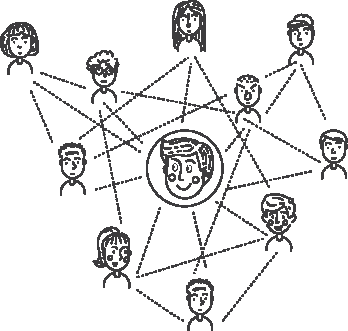
\includegraphics[scale=1.2]{willpower/ch10/7.pdf}
\end{figure}

\emph{Калі ваш сябар пачаў курыць, то ваша рызыка закурыць павышаецца на 61\,\%, у~вашага сваяка нарадзілася дзіця~--- імавернасьць завесьці дзіця ў~вас павышаецца на 15\,\% на бліжэйшыя два гады. Мужчыны, у~якіх калега скончыў жыцьцё самагубствам, маюць у~3,5 разы вышэйшую рызыку суіцыду.}

\textbf{Хваля зьменаў} рухаецца як да нас, так і ад нас. Так ці інакш, мы зьвязаныя з~400 людзьмі на ўзроўні двух поціскаў рукі, і кожны з~гэтых людзей уплывае на нас. Таму важна ня толькі што робіць ваш сябар, але й якія ў~яго сябры. Мы ўплываем на сяброў, яны на сваіх сяброў, тыя~--- на сваіх сяброў~--- так нашы ўчынкі могуць рэальна ўплываць на жыцьцё людзей, якіх мы ніколі ня бачылі. На шчасьце, добрыя звычкі гэтак жа капіююцца і распаўсюджваюцца, як і шкодныя.

\emph{На нас уплывае ня толькі наша назіраньне за сабой, але й назіраньне іншых людзей за намі: і навакольныя, і дыстанцыйныя настаўнікі зьмяняюць нашы паводзіны. Ня толькі жывыя людзі: нават партрэты і проста намаляваныя вочы дзейнічаюць на наш сацыяльны мозг такім жа чынам. Яда ў~прысутнасьці выяваў іншых людзей здаецца смачнейшай, чым звычайна, а~вось шкодныя прадукты губляюць сваю прывабнасьць~--- у~параўнаньні зь ядой на самоце. А выявы людзей, якія рухаюцца, павялічваюць фізычную актыўнасьць.}

Дзелячыся зь сябрамі шчасьлівымі момантамі свайго жыцьця, вы на 9\,\% павялічвае іх імавернасьць шчасьця, а~аповед пра няшчасьці можа прывесьці да зьніжэньня ўзроўню шчасьця на 7\,\%.

\textbf{Ваш настрой уплывае на іншых: прыйдучы да працы ці вярнуўшыся дахаты, прывядзіце сябе ў норму, надайце час псыхалягічнай гігіене. Гэта важна ня толькі для вас, але й для вашых блізкіх.}

\subsection*{З кім ты ясі}

Узьдзейнічаюць на нас і хуткаплынныя кантакты: напрыклад, калі ў~рэстаране ў~афіцыянта залішняя вага, то людзі звычайна зьядаюць больш, у~4 разы часьцей замаўляюць дэсерт і на 17\,\% часьцей алькаголь. Наш мозг схільны прыдумляць гісторыі, зьвязваючы ўсе факты навокал: калі ўсё вакол тоўстыя, то, магчыма, і табе варта назапасіць некалькі кіляграмаў, бо ``быць як усе''~--- гэта камфортна для мозгу і, як ён лічыць, важна для выжываньня. За апошнія два гады жыхары ЗША сталі на 62\,\% часьцей абедаць адны. Добра гэта ці дрэнна? З аднаго боку, пераяданьне сацыяльна заразнае: калі ваш блізкі сябар пакутуе на атлусьценьне, рызыка лішняй вагі ў~вас павялічваецца на 171\,\%, а~імавернасьць своечасова спыніцца ў~час яды ў~кампаніі зьмяншаецца на 60\,\%. Многія людзі знаёмыя з~гэтым эфэктам не па чутках.

\infobox{У пажылых мужчынаў ежа ў~адзіноце (пры наяўнасьці сям'і) у~2,4 разы павялічвае рызыку дэпрэсіі і на 50\,\% рызыку сьмерці.}

Зь іншага боку, яда ў~атачэньні сям'і і блізкіх аказвае магутны ахоўны эфэкт. У цэлым, у~коле сям'і і блізкіх мы ямо менш, але хутчэй, а~ў кампаніі~--- больш, але павольней. Акрамя гэтага, яда ў~коле сям'і і сяброў зьяўляецца магутным інструмэнтам згуртоўваньня, выхаваньня, станоўча ўплывае і на пасьпяховасьць у~школе, і на колькасьць зьяданай гародніны.

\textbf{Дыстанцыёнка.} Многія людзі і кампаніі заўважылі падзеньне крэатыўнасьці і прадуктыўнасьці супрацоўнікаў на дыстанцыёнцы. Людзі~--- істоты сацыяльныя, і на нашы паводзіны моцна ўплываюць іншыя людзі, хто значны для нас, мы схільныя капіяваць іх паводзіны і нават падладжвацца пад чаканьні. Усё гэта стварае сацыяльны ціск, аксытацынавую агульнасьць і ўключае племянныя інстынкты добра працаваць разам у~імя выжываньня. Усё гэта матывуе нас на падкорцы, не вытрачаючы нашы валявыя працэсы. А калі людзей гэтых побач няма, то матывацыя падае і складаней засяродзіцца без сацыяльнага ціску.

Высокапрадуктыўны супрацоўнік павышае прадуктыўнасьць усіх суседзяў на 15\,\% у~радыусе каля 7 мэтраў. Нават самыя слабыя супрацоўнікі шчыруюць на 10\,\% лепей, калі побач працуюць іх калегі. Атрымліваецца, што эфэктыўнасьць распаўсюджваецца па камандзе, валодаючы ``эфэктам пераліву''. Зрэшты, для таксічных людзей тое самае~--- яны прыкметна зьніжаюць эфэктыўнасьць каманды. Атрымліваецца, што, калі за тваёй працай назіраюць, ты аўтаматычна больш сабраны і матываваны паводзіць сябе правільна. Прысутнасьць іншага чалавека аўтаматычна дапамагае вам засяродзіцца і робіць больш уважлівымі.

Гэта можна выкарыстоўваць, каб мяняць звычкі і працаваць у~камандзе ў~цеснай сувязі, напрыклад, наняць сабе куратара. Так худнеюць Weight Watchers і дапамагаюць адно аднаму ананімныя алькаголікі. А пад кіраўніцтвам трэнэра людзі выкладваюцца нашмат мацней, чым калі займаюцца ў~адзіноце. Можна паспрабаваць працаваць у~пастаянным відэакантакце з~камандай на працягу ўсяго працоўнага дня. А можна і пад наглядам незнаёмца, як прапануе, напрыклад, сэрвіс Focusmate.

\subsection*{Пытаньні і заданьні}

1. Ці часта вы капіюеце звычкі іншых людзей?

2. Ці перадаецца ваш настрой навакольным?

3. Як уплываюць на вашую матывацыю людзі вакол вас?


\section{Разьвівайце сацыяльныя навыкі}

Як апэтыт прыходзіць падчас яды, так і радасьць ад камунікацыі прыходзіць падчас размовы. Вядома, ёсьць людзі больш таварыскія, у~працэсе жыцьця ў~кагосьці лепш атрымліваецца заводзіць знаёмствы, хтосьці больш камунікуе і яшчэ больш шліфуе свае навыкі. Іншыя з~раньняга ўзросту саромеюцца, пазьбягаюць камунікацыі, што яшчэ мацней пагаршае гэтыя навыкі,~--- і так фармуецца чарговае заганнае кола. Разьвітыя сацыяльныя навыкі важныя для адаптыўнасьці і нашага фізычнага і сацыяльнага здароўя, робяць нас супэрпрафэсіяналамі і часта даюць магчымасьць прэтэндаваць на самыя прыбытковыя пасады. Посьпех ні да каго не прыходзіць паасобку, таму навыкі фармаваньня каманды і падтрыманьня ў~ёй здаровай сацыяльнай атмасфэры вельмі запатрабаваныя.

\textbf{Эмацыйны інтэлект.} Пачынаецца разьвіцьцё эмацыйнага інтэлекту з~усьвядомленасьці і ўменьня разумець і выяўляць свае эмоцыі. Людзі зь нізкім эмацыйным інтэлектам пакутуюць ад няўпэўненасьці, самакрытычнасьці і ня могуць эфэктыўна ўзаемадзейнічаць з~навакольнымі. Чым лепш вы разумееце самі сябе і дакладней сыгналізуеце аб сваіх намерах іншым, тым лягчэй вас зразумець і прыемней з~вамі размаўляць. Гэта спрыяе зьяўленьню пачуцьця агульнасьці і эфэктыўнай сумеснай рабоце.

\infobox{Эмацыйную пісьменнасьць можна ўмоўна падзяліць на 4 часткі: усьведамленьне сваіх пачуцьцяў, кіраваньне эмоцыямі, суперажываньне, эмацыйная інтэрактыўнасьць.}

\textbf{Уважлівасьць.} У кожным з~нас ёсьць мэханізм разуменьня іншых людзей: мы ўмеем адрозьніваць падман, дакладна ацэньваем людзей, можам бачыць, як яны рэагуюць на нашы словы, і мяняць свой стыль камунікацыі так, каб навакольным было прыемна з~намі размаўляць. Калі мы няўважлівыя да іншых людзей, то не атрымліваем ад іх зваротнай сувязі і нам цяжка палепшыць эфэктыўнасьць камунікацыі. 

\textbf{Назірайце ўважліва за сацыяльным кантэкстам, ацэньваючы дарэчнасьць тых ці іншых паводзінаў.} Улік кантэксту важны, і заўсёды ёсьць падказкі, як лепей паводзіцца тут і зараз. У мяне ёсьць сябар~--- прыроджаны геній камунікацыі, вельмі эмпатычны і гнуткі, які разумее людзей з~аднаго позірку. А вось у~мяне сацыяльная інтуіцыя слабая, я не разумеў невэрбальных сыгналаў і рэакцый іншых людзей. Але самаадукацыя і ўважлівасьць дапамаглі мне яе разьвіць, я стаў нашмат лепш заўважаць рэакцыі іншых людзей і правільней на іх рэагаваць.

\emph{Знайдзіце камунікацыйнага генія і назірайце, як ён камунікуе. Нават простае назіраньне дапаможа вам лягчэй засвоіць гэтыя навыкі, пераймаючы іх. Гэта сапраўды працуе.}

Шчырая ўважлівасьць да іншых нараджаецца зь цікавасьці, а~цікавасьць узьнікае, калі мы знаходзім у~чалавеку нешта важнае для нас, нешта агульнае паміж намі, нейкую рысу, якая робіць чалавека асаблівым, нешта, чаму чалавек можа нас навучыць або чым узбагаціць. Часта адсутнасьць увагі да іншага~--- гэта наша зацыкленасьць на сабе і сацыяльны інфантылізм, неразьвітасьць сацыяльных навыкаў, эгаізм. На жаль, шматлікія людзі лічаць, што іх мэта ў~камунікацыі~--- самапрэзэнтацыя, яны кажуць аб сабе, імкнучыся выказаць сваё меркаваньне і ацэнку, нават не задаючыся пытаньнем, ці трэба гэта суразмоўцу. Вядома, такая манэра выклікае толькі непрыманьне. Сапраўдная камунікацыя~--- гэта ўзаемная цікавасьць, калі абаім размова карысная, цікавая і прыносіць задавальненьне.

\textbf{Важна зацугляць сваю гордасьць} і сфакусавацца на суразмоўцы. Што яму цікава? Пра што ён хоча і пра што ня хоча гаварыць? Што яго непакоіць? Як я магу дапамагчы яму? Што цёплага я магу сказаць і як падтрымаць? Як зрабіць, каб пасьля размовы ў~нас застаўся прыемны посмак? Для адказу на гэтыя пытаньні ў~нас у~мозгу ёсьць адмысловыя цэнтры, якія могуць мадэляваць псыхічны стан іншага чалавека, трэба толькі шчыра зацікавіцца ім. Пастаўце сябе на яго месца: чаму ён так паводзіцца? Паспрабуйце прымерыць на сябе ягоныя эмоцыі. Пакажыце, што разумееце яго. камунікуючы, кажыце не пра сябе, а~пра суразмоўцу.

\emph{Як трапна сказаў доктар філязофіі Уорэн Беньніс: «Калі я паабедаў з~Гладстоунам, то зразумеў, што ён~--- самы разумны чалавек у~сьвеце. Але калі я паабедаў з~Дызраэлі, то зразумеў, што самы разумны чалавек на сьвеце~--- я».}

У любой сытуацыі будзьце ветлівыя з~усімі. Няветлівасьць ня толькі непрыемная для навакольных, яна зьмяншае і ваш сацыяльны статус. Навучыцеся правільна пачынаць і заканчваць размову~--- гэтыя моманты ўплываюць на ўспрыманьне камунікацыі. Пільнуйце асабістыя межы. Калі вас не пытаюцца напрамую, ня ўмешвайцеся, не давайце парадаў, не крытыкуйце. І я ўпэўнены, што заўсёды можна знайсьці нагоду пахваліць чалавека. Пазітыўны стыль камунікацыі матывуе і гуртуе каманду.

\textbf{Камплімэнты і пахвала} павінны быць разумнымі, дарэчнымі, умеранымі і шчырымі, інакш прывядуць да супрацьлеглага эфэкту. Уважліва назіраючы за суразмоўцам, вы зразумееце, што можна пахваліць невідавочнае (напрыклад, камплімэнт пра выгляд у~многіх сытуацыях будзе недарэчным). Напрыклад, тыя рэчы, якія чалавек умее добра рабіць: яго энэргічнасьць і накіраванасьць, экспэртнасьць у~чымсьці, можна падзякаваць яму за цікавую інфармацыю, атачэньне, эмоцыі, якія ён нараджае ў~вас. Таксама важна і прымаць зьвернутыя да вас камплімэнты годна і з~павагай, дзякаваць суразмоўцу.

\emph{Мне зь дзяцінства было псыхалягічна цяжка хваліць людзей і рабіць ім камплімэнты, гэта здавалася штучным, я баяўся падацца навязьлівым. Але аказалася, што гэта проста і прыемна: цяпер хваліць іншых і рабіць ім камплімэнты прыносіць мне самому задавальненьня ня менш, чым тым, да каго зьвернутая пахвала.}

\textbf{Навучыцеся слухаць.} Філёзаф Фрэнсіс Бэкан заўважыў: «Мужчына ўжо напалову закаханы ў~кожную жанчыну, якая слухае, як ён гаворыць». Вы можаце прыкметна палепшыць свае сацыяльныя навыкі, калі навучыцеся актыўна слухаць суразмоўцу. Асабліва ўважліва мы павінны слухаць важнага нам чалавека, перадусім калі ён адчувае моцную эмоцыю або калі ёсьць рызыка ўзьнікненьня непаразуменьняў.

\infobox{Шчырая ўвага ня толькі паляпшае разуменьне, гэта яшчэ і найлепшы камплімэнт. Спытайце сябе: ці адкрыты вы да суразмоўцы, ці адчуваеце да яго цікавасьць?}

\emph{Слухаючы суразмоўцу, я заўсёды імкнуся сфакусавацца на ім, зразумець як мага глыбей ня толькі яго маўленьне, але й эмоцыі і невэрбаліку. Калі я вучыўся ў~мэдыцынскім унівэрсытэце, то выявіў цікаўны пабочны эфэкт гэтай звычкі~--- нават калі я не размаўляў з~выкладчыкам, але ўважліва слухаў яго на занятках і лекцыях, то ён па змоўчаньні пачынаў лічыць мяне разумным і кемлівым яшчэ да таго, як я адкрываў рот на іспыце.}

Вашаму суразмоўцу вельмі важна ведаць, што вы яго разумееце, падзяляеце ягоныя пачуцьці і эмоцыі. Ня трэба сьлепа капіяваць яго гэсты і адлюстроўваць, як часта раяць,~--- проста ўпусьціце ягоныя эмоцыі ў~сябе і вашае цела адрэагуе максімальна дакладна і дарэчна. Ня бойцеся выгараць, прымаючы пачуцьці,~--- спачуваньне і суперажываньне валодаюць ахоўным эфэктам. Так, дасьледаваньне практыкі «мэдытацыя любові й дабрыні» паказала павелічэньне актыўнасьці парасімпатыйнай нэрвовай сыстэмы, якая зьмяншае ўзровень стрэсу.

\textbf{Каб лепш слухаць, спачатку перастаньце гаварыць,} дайце суразмоўцу магчымасьць выказацца. Невыпадкова ў~нас два вухі і адзін рот: мы павінны ня толькі чуць словы, але й разумець пачуцьці суразмоўцы і падтэкст яго паведамленьняў. Для прыхільнае гутаркі стварыце атмасфэру цікавасьці, каб вашаму суразмоўцу было лёгка і вольна: зручна прысядзьце, прычыніце дзьверы, прыглушыце гучную музыку, адключыце тэлефон. Не адцягвайцеся на бытавыя справы, будзьце цярплівыя і спакойныя. Не глядзіце на гадзіньнік, ці тэлефон, ці іншых людзей~--- гэта можа забіць усю цікавасьць. Задавайце пытаньні, а~не крытыкуйце ці спрачайцеся. Паспрабуйце пры камунікацыі забясьпечыць прамы кантакт, загадзя плянуйце час для сяброў і сям'і. Калі ваш час абмежаваны, загадзя абгаварыце тэрмін і папярэдзьце, што сьпяшаецеся, каб не давялося груба перарываць суразмоўцу.

\textbf{Заахвочвайце суразмоўцу}~--- гэта можна рабіць як кіўкамі, так і рэплікамі і праявай эмоцыяў. Для праверкі свайго разуменьня задавайце ўдакладняючыя пытаньні і вяртайце пачутыя словы, перафразуйце іх. Калі вы нечага не разумееце, прызнайце гэта. Пакажыце сваё суперажываньне, падзяліце пачуцьці суразмоўцы. Вытрымлівайце паўзу перад тым, як даць адказ. Абавязкова правільна завяршыце размову: скажыце прыемнае, пазычце посьпехаў, падсумуйце размову і дамоўцеся аб новай сустрэчы. Выяўляйце цікавасьць невэрбалікай: крыху падайцеся наперад, глядзіце ў~твар, рабіце мікрагэсты.

Навучыцеся даваць актыўную канструктыўную рэакцыю ў~камунікацыі. Напрыклад, ваш сябар кажа: «Я пасьпяхова завяршыў праект». Аптымальная рэакцыя: «Крута, ты столькі намаганьняў уклаў у~яго. Я ганаруся табой! Што ты адчуваеш? Давай адсьвяткуем!» На жаль, часта людзі рэагуюць пасіўна «а, прыкольна» ці нэгатыўна «ха-ха, зараз ня будзе чым заняцца».

\textbf{Трэніруйце эмоцыі.} Важна ня толькі разумець, але яшчэ і дакладна выяўляць свае эмоцыі. Складзіце сьпіс эмоцыяў і паспрабуйце іх прымерыць на сябе, як быццам розныя строі. Трэніруйцеся зь люстэркам~--- так вы можаце ярчэй зразумець міміку і невэрбаліку.

\infobox{Чым большы спэктар эмоцыяў і чым дакладней вы іх выражаеце, тым лягчэй вам будзе іх заўважаць не адно ў~сябе, але й у~іншых людзей.}

Паспрабуйце ў~адной эмоцыі абраць найболей пасоўны і прыгожы спосаб яе выразу: зьбярыце фота вашых усьмешак ці вашага суму і прапануйце сябрам вызначыць эмоцыю. Калі яны памыляюцца, значыць, вы недакладна выяўляеце свае эмоцыі і можаце быць няслушна зразуметыя навакольнымі. Навучыцца адчуваць нэгатыўныя эмоцыі таксама важна~--- гэта дапаможа вам быць больш стрыманымі і канструктыўней рэагаваць.

\begin{figure}[htb!]
  \centering
  
\includegraphics[scale=1.5]{willpower/ch10/8.pdf}
\end{figure}

\textbf{Альтруізм.} Горшае, што можна зрабіць,~--- гэта знаёміцца для таго, каб выкарыстоўваць людзей або чакаць ад іх паслуг. Такая стратэгія заўсёды пройгрышная. Камунікацыя~--- узнагарода сама па сабе. Падтрыманьне сувязяў і дапамога іншым людзям у~першую чаргу карысныя для вашага здароўя, а~ўсё астатняе~--- прыемны бонус. Сапраўдная камунікацыя~--- гэта імкненьне зрабіць іншых шчасьлівымі. Пытайце сябе «чым я магу дапамагчы гэтаму чалавеку», а~не «што я магу ад яго атрымаць?».

\textbf{Агульныя інтарэсы.} Не фіксуйцеся на адрозьненьнях, знайдзіце агульнае з~вашым суразмоўцам. Прызнайце безумоўна і безумоўна значнасьць вашага суразмоўцы, усё роўна хто ён. Камунікацыя заўсёды дапамагае нам атрымліваць выдатную зваротную сувязь адносна ўсяго, што мы робім.

\textbf{Падзяка і пахвала.} Выказвайце ўдзячнасьць пры кожным зручным выпадку. Найлепшае ўзьдзеяньне на чалавека~--- гэта заахвочваньне жаданых паводзінаў, а~ня крытыка. Будзьце паблажлівыя і не судзіце іншых людзей, не чакайце асаблівага стаўленьня~--- такія залішнія чаканьні могуць сапсаваць усё задавальненьне ад камунікацыі.

\emph{Звычка да падзякі цудоўна здымае стрэс: нават за ядой мы можам у~думках падзякаваць сотні людзей, чыя праца дапамагла вырасьціць і даставіць прадукты, якія вы ясьце, зрабіць моцны стол, за якім вы седзіце, і пабудаваць дом, дзе вы жывяце.}

\textbf{Прасіце аб дапамозе.} Уменьне зьвяртацца па дапамогу вельмі важнае, бо нашыя сацыяльныя сувязі сапраўды могуць нам дапамагчы~--- эмацыйна, інфармацыйна і мноствам іншых спосабаў. Ня бойцеся прасіць аб гэтым, бо для многіх людзей пасільная дапамога сапраўды прыемная, і яны з~задавальненьнем паспрыяюць вырашэньню вашых праблемаў. Прасіце правільна: знайдзіце чалавека, прыцягніце яго ўвагу і выразна апішыце вашу праблему. Выкажыце свае пачуцьці адносна гэтай сытуацыі, удакладніце, чаго б вы хацелі. І затым апішыце магчымыя наступствы. Калі вам дапамагаюць, прымайце гэта годна, падкрэсьліце ролю чалавека і важнасьць яго ўдзелу, дзякуйце.

\infobox{Вы і вашыя знаёмыя фармуеце сыстэму ўзаемных сувязяў~--- калі ўсе яе ўдзельнікі адчуваюць неабходнасьць адно ў~адным, гэта ўзбагачае кожнага з~вас.}

\textbf{Позірк вочы ў~вочы і аксытацын.} У наш век смартфонаў мы глядзім адно на аднаго нашмат менш. Хочацца, каб мы падарылі сваім каханым і блізкім нешта большае, чым падарункі~--- падарылі ім свой чысты час, сваю шчырую ўвагу і позірк вочы-ў-вочы. Нашыя вочы створаныя для камунікацыі. Белая цьвердавіца чалавечага вока разьвілася зь неабходнасьці адсочваць рухі вачэй і кірунак позірку. Людзі валодаюць найбольшымі суадносінамі адкрытай цьвердавіцы ў~контуры вока, і наш контур вачэй гарызантальна падоўжаны. 

\emph{Нованароджаныя ўжо зь пяці дзён адсочваюць позірк і адрозьніваюць, калі ім глядзяць у~вочы. У дзяцей погляд вочы-ў-вочы стымулюе разьвіцьцё сацыяльных навыкаў, маўленчай памяці.} 

Калі мы ўсталёўваем позірк вочы-ў-вочы, гэта запускае ў~нашым мозгу магутныя зьмены: узмацняецца актыўнасьць «сацыяльнага мозгу», пярэдняй зьвіліны поясу, мозачкаў, лімбічнай сыстэмы, люстраных нэўронаў. Мы становімся больш адчувальныя і эмпатычныя, позірк «разагравае» нас для камунікацыі, павялічвае самаўсьвядомленасьць. Падсьвядома запускаецца «аўтаматычная мімікрыя», калі людзі сынхранізуюць свае рухі вачэй, утвараючы «танец» поглядаў, калі вытрымліваюцца дастатковая частасьць і працягласьць позіркаў. Па меры росту даверу працягласьць кантакту плаўна ўзрастае. Тыя, хто праходзіць гэты тэст візуальнай сынхранізацыі, могуць прэтэндаваць і на бліжэйшую камунікацыю.

\textbf{Калі вы гледзіце, узровень аксытацыну расьце}, вам прыемна і хочацца працягваць глядзець у~вочы, часьцей дакранацца, быць побач. Так фармуюцца доўгатэрміновыя завесы прыхільнасьці ў~бацькоў і дзяцей, закаханых, сабакі і яго гаспадара. Упэўнены, многія з~вас адчувалі прыемнае галавакружэньне ад доўгага позірку каханага чалавека. А вось калі чалавек пазьбягае позірку, аксытацын зьніжаецца, вам менш хочацца шукаць кантакт і глядзець на чалавека, і сувязь паміж вамі слабее~--- такім чынам закручваецца так званая адмоўная аксытацынавая пятля. Мы ацэньваем тых людзей, хто падтрымлівае з~намі прыязны кантакт вачыма, як больш разумных і шчырых, больш верым таму, што яны гавораць.

\emph{Дасьледаваньні паказваюць, што незнаёмцы, зь якімі мы ўстанавілі прыязны глядзельны кантакт, ацэньваюцца як больш «падобныя», «якія маюць нешта агульнае з~намі».}

Аднак доўгі позірк ад чужых людзей выклікае варожасьць. Аксытацын узмацняе жаданьне абараняць сваіх і можа стымуляваць нанясеньне «апераджальных удараў» па чужынцах з~мэтай абароны ад магчымай агрэсіі зь іх боку. Працяглы кантакт расцэньваецца як уварваньне ў~асабістую прастору. 

\textbf{Пры статусных сутыкненьнях доўгі позірк зьяўляецца выклікам, а~здольнасьць вытрымаць пільны позірк іншага чалавека~--- паказьнікам сілы.} 

Самы вялікі падарунак на сьвяты і ня толькі, які мы можам зрабіць сваім блізкім,~--- гэта чыстая ўвага і суперажываньне, што немагчыма без глядзельнага кантакту. Адкладзіце тэлефоны і часьцей глядзіце на каханых, адказвайце на зьвернутыя на вас позіркі, фармуйце станоўчыя аксытацынавыя сувязі.

\subsection*{Пытаньні і заданьні}

1. Ці заўсёды навакольныя дакладна разумеюць вашыя эмоцыі? Ці добра вы ўлоўліваеце сацыяльны кантэкст?

2. Ці часта вы робіце камплімэнты і хваліце іншых людзей?

3. Наколькі ўважліва вы ўмееце слухаць суразмоўцу?


\section{Асабістыя межы}

Больш за дзьве тысячы гадоў таму ў~Атэнах зарадзіўся рух стаіцызму. Яго інтэлектуальная спадчына~--- кнігі Сэнэкі, Эпіктэта і Марка Аўрэлія~--- прачытаныя мною ў~поўным аб'ёме. Мой малодшы сын атрымаў імя Марк не ў~апошнюю чаргу дзякуючы філёзафу-імпэратару, чыя кніга часта ляжала ў~мяне на працоўным стале. Адной з~найважнейшых ідэй стаіцызму было ўменьне адрозьніваць, што мы можам кантраляваць, а~што~--- не, і праводзіць мяжу паміж гэтым. Мужна мяняць тое, на што мы можам узьдзейнічаць, і прымаць тое, на што мы ня здольныя паўплываць.

Наш мозг па-рознаму рэагуе на падзеі ў~залежнасьці ад таго, ``нашымі'' ці ``ня нашымі'' ён іх лічыць. ``Нашым'' мозг лічыць тое, што ідэнтыфікуе з~сабой, чым можа кіраваць. У сваю псыхалягічную прастору ўваходзіць ня толькі цела, мы можам уключаць у~сваю схэму ўплыву і свае звычкі, ідэі, рэчы, іншых людзей і рэагаваць так, быццам гэта часткі нашага сапраўднага ``Я''. З узростам і ростам усьвядомленасьці, пазбаўляючыся ад інфантылізму, чалавек разумее, што ў~іншых людзей ёсьць свае межы, жаданьні і адчуваньні. 

Мы разумеем, што можам уплываць на свае думкі і дзеі і што ня варта ўмешвацца ў~чужыя межы, спрабуючы зьмяніць думкі і дзеі іншых людзей. Разумеем, але ня ўсе і не заўсёды, і тэма асабістых межаў цяпер вельмі актуальная, мы ўсё часьцей ужываем словы: таксічныя стасункі, хэйт, абясцэньваньне, газлайтынг. Марку Аўрэлію такое і ня сьнілася.

\textbf{Здаровыя асабістыя (псыхалягічныя) межы}~--- гэта разуменьне ўласнага ``Я'' як асобнага ад іншых, разуменьне ўласных межаў і межаў іншых людзей, уменьне вырашаць жыцьцёвыя задачы самастойна. Гэтае разуменьне дазваляе эфэктыўна будаваць узаемадзеяньне: з~аднаго боку, чалавек можа лёгка адмовіць, з~другога~--- не навязваецца. Здаровыя межы ў~камунікаваньні~--- гэта ўзаемная цікавасьць, а~не калі адзін з~удзельнікаў прымушае іншых людзей рабіць ці слухаць тое, чаго яны ня хочуць і што ім нецікава.

У любой сытуацыі важна выразна і сьвядома разьмежаваць тое, што ўсярэдзіне вашага локусу і што звонку. Напрыклад, пры канфлікце вы ня можаце кантраляваць эмоцыі і паводзіны іншага чалавека, а~можаце~--- свае дзеі і рэакцыю. Процілегласьць кантролю~--- гэта бездапаможнасьць, калі чалавек наогул адмаўляецца браць кантроль за свае ўчынкі ды імкнецца сьпісваць усё на навакольныя чыньнікі й іншых людзей. Калі чалавек ня бачыць межаў, то ягонае сьветаўспрыманьне становіцца зьмененым~--- ён ня можа адрозьніць уласныя імпульсы і жаданьні ад індукаваных звонку, а~таксама праецыруе свае жаданьні на навакольных. Калі такому чалавеку нехта падабаецца, то ён адчувае ілюзію, што суразмоўца таксама адчувае да яго сымпатыю. Калі такі чалавек хоча выпіць, то яму здаецца, што гэта бутэлька кліча яго.

\textbf{Ня ўмешвайцеся ў~чужыя межы.} Здаровыя межы~--- гэта безумоўнае безацэннае прыняцьце іншых людзей і іх асаблівасьцяў. У разьдзеле ``Усьвядомленасьць'' мы разабраліся, чаму прыняцьце такое важнае,~--- яно дапамагае пазьбегнуць канфлікту вашых чаканьняў і рэальнасьці. Калі мы не паважаем і не прымаем межы іншых людзей, то парушаем іх умяшаньнем: крытыкуем, выказваем сваё «меркаваньне», даем няпрошаныя парады, дапамагаем ці вырашаем нешта за іншых. 

\textbf{Спыніцеся.} Спытайце сябе, ці прасілі вас пра гэта, ці сапраўды гэта трэба чалавеку? Калі вы парушаеце межы іншых людзей, то змушаеце іх абараняцца і нападаць на вас, пагаршаючы камунікацыю. Адзіны чалавек, чыю рэакцыю, думкі і паводзіны вы можаце кантраляваць,~--- гэта толькі вы самі.

\textbf{Адрозьнівайце, што вашае, а~што ня вашае.} Гіпэркантроль і гіпэрапека~--- гэта кепска. Калі вы карыстаецеся слабасьцю іншых людзей, у~канчатковым выніку такое ўварваньне будзе шкоднае і для вас. Нават калі вы дамагліся свайго, здушыўшы іх волю і супраціў,~--- гэта нездаровыя адносіны і яны ня пойдуць вам на карысьць у~доўгатэрміновай пэрспэктыве.

\emph{Трэба быць уважлівымі і задаваць сабе пытаньні пра межы асабістай прасторы іншага. Ці хоча чалавек вас слухаць? Ці трэба вам умешвацца ў~чужую размову? Навошта вы рабілі чужую працу, хаця вас пра гэта й не прасілі? Ці ўмешваліся вы ў~баўленьне часу іншых без апавяшчэньня або іх жаданьня? Тэлефанавалі позна, пісалі недарэчна?}

Вы можаце распаўсюджваць свае межы на непадуладныя вам задачы і людзей, уключаючы іх у~сваё псыхалягічнае «цела» і затрачваючы неймаверную колькасьць энэргіі на спробы кантролю або перажываньні. Напрыклад, берацеся за задачу, рашэньне якой ад вас не залежыць, намагаецеся~--- але ў~гэтым няма сэнсу. 

\textbf{Прыкмета здаровых межаў}: вы не бераце на сябе чужы груз, ня лезеце ў~чужую справу, берацеся за тое, на што можаце ўплываць. Дзейнічайце экалягічна: сумленнасьць з~сабой і навакольнымі, адмова ад эмацыйнага і фізычнага гвалту, адмова ад падману і маніпуляцый. Многія людзі лічаць, што іх пакуты, перажываньні, меркаваньні маюць каштоўнасьць для навакольных. На жаль, гэта ваша ілюзія, што навакольныя абавязаны выслухоўваць усё, што з~вас ліецца. Ня варта дзяліцца сваімі траўмамі і страхамі з~усімі навакольнымі~--- такая споведзь ахвяры нікому не цікавая. Калі вы зьвяртаецеся да іншых, то ваша прапанова павінна быць прывабнай, а~не выклікаць адрынаньне. Не рабіць і не балбатаць лішняга~--- выдатная крыніца сілаў і энэргіі. Спытайце сябе, ці будзе цікавая тая ці іншая інфармацыя вашаму суразмоўцу? Калі не разумееце, што яму цікава, то спытайце прама.

\begin{figure}[htb!]
  \centering
  
\includegraphics[scale=1.5]{willpower/ch10/9.pdf}
\end{figure}

\textbf{Абараняйце свае межы.} Псыхалягічныя межы падобныя межам клетак арганізма: яны прапускаюць карысныя рэчывы і блякуюць пранікненьне шкодных. Абарона асабістых межаў~--- гэта сьвядомы допуск іншых людзей да ўнутраных перажываньняў, і толькі вы вырашаеце, хто, як і калі будзе з~вамі ўзаемадзейнічаць. Важна дакладна выяўляць свае (не)жаданьні і ўмець адмаўляць, казаць ``не'' экалягічна і своечасова.

\infobox{Не прымушайце сябе выслухоўваць нецікавыя рэчы, умейце выразна паказваць, калі вам нешта ня трэба ці некарысна.}

Вучыцеся адсочваць, калі нехта спрабуе прымусіць вас нешта зрабіць рознымі спосабамі: маніпулюючы пачуцьцём віны, прымушаючы, запалохваючы і да т.~п. Калі людзі не прымаюць вашыя ўмовы камунікацыі ды ігнаруюць вашыя запыты~--- спыняйце такую камунікацыю. Здаровыя межы абараняюць ад залежных адносінаў і дазваляюць не прымаць адказнасьць за тое, як сябе паводзяць ці пачуваюцца іншыя людзі. Ня бойцеся наступстваў адмовы, што на вас прытояць нейкую крыўду ці што бяз вас усё пойдзе ў~глум~--- гэта перабольшаньні.

\emph{Ня ўмееце казаць «не»? Мастацтву ветліва адмаўляць прысьвечаны розныя кнігі.}

Мы жывём у~гэтым сьвеце не для таго, каб адпавядаць чаканьням іншых людзей, а~іншыя людзі~--- не для таго, каб адпавядаць нашым. Сыходзьце ад чужых праблемаў, але не з~дапамогай контратакі. Найлепшая абарона~--- гэта не падпарадкоўвацца чужым патрабаваньням і заставацца ва ўласных межах. Крыху ніжэй мы падрабязна пагаворым пра «ўсьвядомленае непадпарадкаваньне».

\textbf{Выкладайцеся максімальна ў~сваіх межах.} Галоўнае~--- не мяжа, а~тое, што ўнутры. Для таго каб межы функцыянавалі аптымальна, важна ўмець самастойна вырашаць бягучыя задачы, спраўляцца з~эмацыйнымі выклікамі, рэгуляваць свой стан. На жаль, многія людзі так і не пераадолелі інфантыльнасьць, таму замест вырашэньня сваіх праблемаў чакаюць, што нехта прыйдзе і вырашыць іх пытаньні. Многія людзі маюць настолькі слабыя межы, ажно амаль зьліваюцца з~навакольнымі, чакаючы ад іх дапамогі і дзеяў, і жывуць у~пошуку ``збаўцы''. Чым больш абавязкаў або чаканьняў вы перакладаеце на іншых людзей, тым больш гэта забірае сілаў у~вас: даводзіцца ўпрошваць, ціснуць ці маніпуляваць для атрыманьня жаданага.

\infobox{Маніпуляцыі не працуюць, толькі вы самі можаце сябе па-сапраўднаму выратаваць~--- хоць бы як багор Мюнхгаўзэн, які выцягнуў сябе за валасы з~багны.}

\textbf{Будзьце сьціплыя.} Разуменьне сваіх межаў і абмежаваньняў дазваляе ставіць сабе задачы, адэкватныя вашым сілам. Сьціпласьць~--- гэта ўсьведамленьне і кантроль тых рэсурсаў, якімі вы валодаеце ў~сапраўдны момант, то бок мы жывём ``па сродках'', а~ня просім ці патрабуем дапамогі. Розныя ілюзіі адносна сябе і сваіх магчымасьцяў і псыхалягічныя абароны размываюць і затуманьваюць межы. Самаацэнка многіх людзей не зьяўляецца прадуктам іх унутранага локусу і задавальненьня ад зробленай працы, а~завязаная толькі на іншых людзях. Калі вы ня можаце хваліць сябе, то пачынаеце жыць дзеля пахвалы іншых. 

\textbf{Сацыяльная ўхвала}~--- гэта наркотык, калі яна становіцца асновай для вашага жыцьця. Зьмяненьне харчаваньня, трэніроўкі дзеля фатаграфіі ў~інстаграме вырачаныя на правал у~доўгатэрміновай пэрспэктыве: як толькі вонкавая ўхвала аслабла, чалавек адразу кідае заняткі. 

\textbf{Сапраўдная супэрсіла}~--- гэта калі вы пачалі бегаць або запусьцілі новы праект, і нікому не сказалі. Няхай за вас гавораць справы, а~ня словы. Будзьце самі сабе настаўнікамі: хваліце сябе за працу, за прагрэс. Няхай у~вас будзе шмат асабістых таямніц, пра якія навакольныя ня ведаюць. 

\subsection*{Пытаньні і заданьні}

1. Наколькі добра вы разумееце межы іншых людзей?

2. Ці ўмееце вы ветліва абараняць асабістыя межы?

3. Ці часта вы выходзіце за асабістыя межы?


\section{Небясьпекі сацыяльнага асяродзьдзя}

Камунікацыя дае шмат плюсаў, але можа быць і крыніцай праблемаў. Мы ўжо разабраліся зь небясьпекай сацыяльнага заражэньня, але высокі ўзровень згуртаванасьці можа прывесьці і да таго, што мы будзем схільныя падпарадкоўвацца групе. Нашы продкі жылі ў~маленькіх згуртаваных групах і варагавалі зь іншымі групамі, так адбываўся міжгрупавы адбор. Менавіта таму нашы найлепшыя якасьці шчыльна зьвязаныя з~горшымі. Так, альтруізм у~людзей першапачаткова быў накіраваны толькі на чальцоў сваёй групы і разьвіваўся ў~адзіным комплексе з~варожасьцю да чужынцаў. 

\emph{Аксытацын выклікае добразычлівае стаўленьне да іншых людзей, дазваляе верыць словам канкрэтнага чалавека, аднак гэта стасуецца толькі ўнутрыгрупавых адносінаў. Адначасова аксытацын стымулюе памяншэньне даверу да староньніх і ўзмацненьне культурных і расавых забабонаў.}

Многія людзі гатовы ахвяраваць сваімі інтарэсамі, то бок зьдзейсьніць альтруістычны ўчынак дзеля сваіх. Пры гэтым яны часта зь ня меншай гатоўнасьцю ідуць на ахвяры дзеля таго, каб нашкодзіць прадстаўнікам варожых груп. Ваенныя подзьвігі і дзеяньні тэрарыстаў-самазабойцаў~--- тыповыя прыклады такіх паводзінаў. У чалавечых грамадствах альтруістычныя дзеяньні абодвух тыпаў, як правіла, высока цэняцца, лічацца «высокамаральнымі», «гераічнымі», «патрыятычнымі» і да т.~п. На гэтым пабудаваная большая частка прапаганды.

\textbf{У моцна згуртаванай групы} ёсьць і іншыя мінусы. Калі вы не выконваеце правілы групы або пярэчыце прынятым большасьцю рашэньням, то група можа гуртавацца супраць вас і перашкаджаць вам дамагацца асабістых мэтаў.

\emph{Ведаеце, адкуль бярэцца страх публічнага выступу? Калі вы стаіце перад «зграяй», вылучаючыся сярод астатніх, і мноства пар вачэй накіравана толькі на вас, ёсьць генэтычны страх «быць зьедзеным» за думку ці ідэю, зь якой можа быць ня згодная большасьць. Бо той, хто кінуў выклік важаку або зграі, караўся выгнаньнем.}

У закрытых групах высокі сацыяльны кантроль, гэта абрывае іншыя сувязі і абмяжоўвае вас. Больш за тое, у~групе могуць пачаць распаўсюджвацца свае небясьпечныя правілы, якія ігнаруюць грамадзкія нормы: часта групавая салідарнасьць толькі ўмацоўвае намер жыць насуперак астатняму грамадзтву. Павышэньне даверу ўнутры такой групы зьніжае давер да навакольнага сьвету. Многія сэкты і закрытыя супольнасьці небясьпечныя для сваіх удзельнікаў.

\subsection*{Статкавы інстынкт}

Для захаваньня ўстойлівасьці і аўтаноміі вельмі важна вытрымліваць сацыяльны ціск і ўмець супраціўляцца статкаваму інстынкту. Для нашага мозгу адрозьнівацца ад навакольных~--- гэта паводзінная памылка. Мозг заўжды дае нам зразумець, калі нашы дзеяньні ці меркаваньні супярэчаць навакольным, і мы пачуваемся вельмі некамфортна. А вось зьмена меркаваньня на агульнапрынятае прыносіць палягчэньне~--- але ня факт, што гэта правільна.

\infobox{У працэсе эвалюцыі, калі вонкавыя ўмовы былі пастаяннымі, адхіленьне ад паводзінаў групы магло каштаваць жыцьця: усе бягуць~--- і я бягу, усе выжылі ці ўсе загінулі.}

Таму ў~стабільных умовах або сыстэмах меркаваньне большасьці можа быць слушным. Напрыклад, эмоцыі людзей не мяняюцца, таму антычныя кнігі да гэтага часу нам цікавыя і ўтрымліваюць мноства карысных для нас ідэй. А вось калі асяродзьдзе новае ці хутказьменлівае, тут канфармізм будзе зусім не адаптыўны.

\textbf{Асабліва ўразьлівыя падлеткі.} Падчас пераходнага пэрыяду яны заклапочаныя меркаваньнем аднагодкаў, вельмі адчувальныя да таго, як да іх ставяцца і што пра іх думаюць іншыя людзі, гостра рэагуюць на сацыяльны ціск, плёткі. Камунікацыя для падлеткаў~--- гэта крыніца задавальненьня і дафаміну, які падштурхоўвае іх да рызыкоўных паводзінаў. Важна разумець гэта, каб дапамагчы падлеткам прайсьці пэрыяд сталеньня бяз стратаў. Бо найлепшы час для фармаваньня сацыяльных сувязяў~--- 18--25 гадоў.

\emph{«Эфэкт аднагодка»~--- калі за падлеткам назіраюць яго сябры, у~яго выдзяляецца больш дафаміну, чым пры тым жа дзеяньні, калі ён знаходзіцца адзін. У дарослых гэты эфэкт зьнікае. Таму падлеткі такія залежныя і адчувальныя да меркаваньня аднагодкаў.}

\textbf{Сацыяльны ціск.} Грамадства зацікаўленае ў~захаваньні стабільнасьці, таму заўсёды выкарыстоўвае мэханізмы ціску на тых, хто не падпарадкоўваецца агульнапрынятым нормам. Падобны кансэрватызм валодае і ахоўным эфэктам, засьцерагаючы ад небясьпечных новаўвядзеньняў. Падабаецца нам ці не, але сацыяльная ацэнка вельмі моцна ўплывае на нашы паводзіны. Мы імкнёмся заслужыць ухвалу і пазьбегнуць асуджэньня. Многія людзі спрабуюць рабіць усё, каб навакольныя былі пра іх «добрай думкі», або скарачаюць зносіны, адмаўляюцца ад праектаў і новых справаў толькі праз тое, каб пазьбегнуць крытыкі або неўхваленьня навакольных.

Важна памятаць: мы маем права ставіць свае інтарэсы вышэй за інтарэсы іншых людзей (не кранаючы пры гэтым іх асабістыя межы), мы маем права памыляцца і адчуваць самыя розныя пачуцьці, нават калі грамадзкая думка вызначае іх як «сацыяльна непрымальныя». Прызнавайцеся сабе шчыра, калі вы ўзрушаныя або злуяцеся. Мы можам і нават абавязаныя мяняць сваё меркаваньне, калі адкрыліся дадатковыя абставіны, і паважаць меркаваньне большасьці ці паважаных чальцоў грамадзтва мы павінны не таму, што яны паважаныя ці іх большасьць, а~з аб'ектыўных аргумэнтаў.

\subsection*{Таксічныя людзі}

Чым больш людзей лезе ў~ваша жыцьцё, тым хутчэй яно дае расколіну: сапраўды, у~сьвеце ёсьць вялікая колькасьць людзей, якія імкнуцца, сьвядома ці неўсьвядомлена, парушаць межы навакольных, маніпуляваць эмоцыямі, палохаць або зьневажаць. Для абароны~--- перахапляйце кантроль у~размове, мяняйце тэму, гаварыце пра суразмоўцу, а~не пра сябе. Можна выкарыстаць вядомы аргумэнт прафэсара Праабражэнскага: ``Проста не хачу''. Не пускайцеся ў~тлумачэньні~--- маніпулятары прымаюць гэта за праяву слабасьці. Дасьледаваньні паказалі, што калі ўкараніць у~каманду аднаго чалавека зь неканструктыўнымі паводзінамі, то яе эфэктыўнасьць упадзе на 30--40\,\%. Таму важная ня толькі наяўнасьць моцных удзельнікаў, але й адсутнасьць слабых. Сярод людзей, зь якімі вы камунікуеце, адзначце тых, зносіны зь якімі робяць вас шчасьлівымі і натхняюць, і тых, хто толькі выцягвае вашу энэргію. Заплянуйце канкрэтныя крокі, каб павялічыць час камунікацыі зь першымі, а~з другімі~--- максімальна скараціць і фармалізаваць.

\textbf{Крытыка.} Многія людзі вельмі гостра ўспрымаюць крытыку, але гэта неад'емная частка нашага жыцьця. Бывае дэструктыўная крытыка, накіраваная супраць нас асабіста і звычайна эмацыйна афарбаваная, яна абясцэньвае нас, факусуецца толькі на нэгатыўных аспэктах, не дае шанцу выправіць. Але крытыка можа быць і канструктыўнай, па сутнасьці~--- звычайнай зваротнай сувязьзю. Часьцей за ўсё яна скіраваная на вырашэньне праблемы, а~ня супраць вас, нясе пазітыўны зарад, дае магчымасьць выправіць, падбадзёрвае і натхняе на вырашэньне праблемы.

Калі крытыка дэструктыўная, то не ўзмацняйце праблему, абараняючыся ці крытыкуючы апанента. Бо крытыкаваць вас могуць і не за справу, а~толькі спрабуючы зацьвердзіцца за ваш кошт. Вы можаце перапыніць размову, падкрэсьліць нязгоду ці сказаць, што ў~вольны час падумаеце над пачутым. А калі вам камфортней~--- можаце і праігнараваць сказанае. Калі вы сапраўды памыліліся, то прызнайце віну і выбачыцеся. Падзякуйце за заўвагу і падрабязна распытайце чалавека. Так ці інакш, вы маеце права на памылку: не памыляецца толькі той, хто нічога ня робіць. А ўменьне сумленна прызнаць свае памылкі і выправіць іх~--- гэта рыса сапраўды ўпэўненага ў~сябе чалавека.

\begin{figure}[htb!]
  \centering
  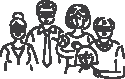
\includegraphics[scale=1.5]{willpower/ch10/10.pdf}
\end{figure}

\infobox{Сярод людзей, зь якімі вы маеце зносіны, адзначце тых, камунікаваньне зь якімі робіць вас шчасьлівей і натхняе, і тых, хто толькі выцягвае вашу энэргію. Заплянуйце пэўныя крокі, каб павялічыць час камунікаваньня зь першымі, а з другімі~--- максымальнае скараціць і фармалізаваць.}

\textbf{Фэномэн падпарадкаваньня.} Навукоўцы лічаць, што схільнасьць да падпарадкаваньня сфармавалася ў~працэсе эвалюцыі і закладзена ў~нас генэтычна, бо выжывалі найбольш зладжаныя групы, якія падпарадкоўваюцца сваім лідэрам. Наогул падпарадкаваньне аўтарытэту, няхай гэта будзе старэйшыя па ўзросьце людзі, бацькі, прадстаўнікі ўлады ці рэлігіі, лічыцца дабрадзейнасьцю і выхоўваецца з~самага дзяцінства ў~пераважнай большасьці культур. Апроч эвалюцыйнай схільнасьці, мы праходзім велізарную школу падпарадкаваньня ў~дзіцячым садку, школе, войску. Усе гэтыя структуры, так ці інакш, прымушаюць душыць свае жаданьні і імпульсы, абясцэньваюць уласную думку і ініцыятыву. Магчыма, ніхто спэцыяльна такой мэты ня ставіць, але ў~сукупнасьці ўсе выхаваўчыя сродкі моцна душаць волю чалавека. \textbf{У выніку многія дарослыя людзі аўтаматычна падпарадкоўваюцца любому, хто ўяўляецца ім аўтарытэтам.}

Мы недаверліва ставімся да гэтага факту і лічым, што зможам запярэчыць злачыннаму загаду, але рэальнасьць~--- кусаецца. Прыклад фашысцкай Нямеччыны паказвае, што ўсяго за некалькі гадоў можна без прамой прынукі прымусіць людзей выконваць самыя жудасныя рэчы дзеля ``агульнага дабра''. Пры гэтым большасьць сама бярэцца за працу, бо яны ``нічога такога ня робяць, а~толькі выконваюць загад''. У пасьляваенныя гады шырокае дасьледаваньне фэномэну падпарадкаваньня пачаў псыхоляг Стэнлі Мілгрэм, які паказаў, што большасьць людзей, падпарадкоўваючыся нават выдуманаму аўтарытэту, нанясуць іншаму чалавеку прамую шкоду, аж да сьмяротнай.

\textbf{Чым вышэйшая схільнасьць згаджацца}, тым вышэйшая рызыка злоўжываньня ўладай, карупцыі і скажэньня рэальнасьці. Лідэр, які звыкся дамагацца сьляпога падпарадкаваньня, неўзабаве губляе сувязь з~рэальнасьцю і, пазбавіўшыся зваротнай сувязі, пачынае рабіць усё больш памылак. Калі лідэр бярэ ўсю адказнасьць і ініцыятыву на сябе, то яго падначаленыя, адпаведна, будуць паводзіць сябе безадказна і безыніцыятыўна. 

\infobox{Маўклівая згода большасьці зьяўляецца тым грунтам, дзе гіне магчымасьць разьвіцьця: прымушаючы і запалохваючы, не чакайце ад працаўнікоў паляпшэньняў, ідэяў і прарыўных рашэньняў.}

Вядома, уменьне падпарадкоўвацца і дакладна выконваць распараджэньні вельмі важнае для эфэктыўнай працы складаных сыстэм. Без лідэра і адзінаначальля праца арганізацый і кампаній можа быць паралізаваная бясконцым абмеркаваньнем і аналізам. Але падпарадкаваньне павінна быць не сьляпым, а~ўсьвядомленым, а~ў процівагу павінен быць разьвіты навык усьвядомленага непадпарадкаваньня. 

\textbf{Усьвядомленае непадпарадкаваньне}~--- гэта ўменьне пярэчыць загаду, застаючыся ў~рамках правілаў і ветлівасьці. Так будучыя навукоўцы павінны спазнаць крытычнае мысьленьне, студэнты~--- уступіць у~дыскусію з~выкладчыкам, пілёты самалёта~--- умець аспрэчваць загады капітана.

\emph{Аналіз шэрагу авіякатастрофаў паказаў, што іх прычынай быў загад капітана, а~другі пілот, які меў пярэчаньні, баяўся іх выразна выказаць і абараніць сваё меркаваньне. Таму ў~сучасных навучальных праграмах усіх чальцоў экіпажу вучаць выяўляць дастатковую настойлівасьць, каб прыцягнуць эфэктыўна вырашаць узьніклыя праблемы.}

Любы лідэр, калі ён сапраўды ўпэўнены ў~сваіх сілах і хоча разьвіцьця сваёй арганізацыі, зацікаўлены ў~тым, каб мець перад сабой адэкватную карціну сьвету і зваротную сувязь, каб яго падначаленыя ўмелі сьвядома падыходзіць да выкананьня задач. Гэта можа зьберагчы ад сур'ёзных памылак.

\emph{У кнізе «Усьвядомленае непадпарадкаваньне» Айра Чэйлаф прыводзіць прыклад з~новенькай медсястрой, якая атрымала загад увесьці прэпарат. Сястра ведала, што ён можа быць фатальны ў~гэтым выпадку, і сказала пра тое лекару, на што атрымала адказ ``ня ваша справа, уводзьце''. Не ўступаючы ў~прамы канфлікт, яна падрыхтавала кропельніцу і зьвярнулася да лекара, каб ён асабіста адкрыў заціск на ёй, бо яна ня будзе гэтага рабіць праз магчымыя ўскладненьні. Гэтага было дастаткова, каб лекар прыслухаўся і зьмяніў сваё меркаваньне.} 

У паўсядзённым жыцьці чалавек з~уладай і аўтарытэтам можа прасіць ці патрабаваць, каб вы зрабілі нешта дрэннае, кіруючыся нават добрымі намерамі. Спытайце сябе, ці мае гэты аўтарытэт дастатковую кампэтэнтнасьць і ці легітымны ён? Выкананьне гэтага распараджэньня прынясе карысьць ці шкоду? Да ўсьвядомленага непадпарадкаваньня трэба падыходзіць творча: можна запытаць загад у~пісьмовым выглядзе або прыводзіць меркаваньне іншых аўтарытэтаў. Знаходзьце саюзьнікаў і пачынайце пярэчыць як мага раней, да фармулёўкі канкрэтнага заданьня ці загаду. Прымаючы рашэньне аб выкананьні, арыентуйцеся на вышэйшыя каштоўнасьці, не дазваляйце ветлівасьці ці субардынацыі прымусіць вас пагадзіцца. Удакладняйце загад, ацэньвайце яго бясьпеку, законнасьць і практычнасьць і прапануйце альтэрнатыўныя магчымасьці і сцэнары.

\infobox{Прымаючы рашэнне, не падпарадкоўвайцеся чужому аўтарытэту безумоўна. Пры гэтым заставайцеся ў~рамках правілаў і ветлівасьці, а~не пераходзіце ў~адкрыты бунт.}

Як часта мы рабілі нешта не таму, што хацелі, а~таму, што нехта сказаў? Як бы нам ні хацелася перакласьці адказнасьць за дзеі на іншых, яна заўжды ляжыць на нас. Кошт падпарадкаваньня ў~нашым жыцьці нашмат вышэйшы, чым здаецца.

\emph{Займаючыся выхаваньнем сваіх дзяцей, вучыце іх ня слухацца~--- і рабіць гэта канструктыўна. Замест таго, каб патрабаваць абсалютнага падпарадкаваньня, пытайцеся, чаму вы просіце іх гэта зрабіць, якія ёсьць іншыя спосабы зрабіць гэта, што здарыцца, калі гэта ня будзе зроблена? Мадэлюйце сытуацыі або гульні, калі аўтарытэту падпарадкоўвацца катэгарычна нельга.} 

\textbf{Асабістая адказнасьць}~--- гэта цяжкі груз, але адначасова і надзейны падмурак. У канчатковым выніку, ад сьляпога падпарадкаваньня ў~сьвеце больш жахаў і сьмерцяў, чым ад бунтаў. Вучыцеся рабіць правільна, выхоўвайце пачуцьцё асабістай свабоды, і, як напісаў Антон Паўлавіч Чэхаў, «гэты малады чалавек выціскае зь сябе па кроплях раба і як ён, прачнуўшыся адной цудоўнай раніцай, адчувае, што ў~яго жылах цячэ ўжо ня рабская кроў, а~сапраўдная чалавечая».

\subsection*{Пытаньні і заданьні}

1. Ці атрымліваеце вы задавальненьне ад прыналежнасьці да нейкай сацыяльнай групы?

2. Ці моцна на вас узьдзейнічае сацыяльны ціск вашага атачэньня?

3. Ці цяжка вам супраціўляцца аўтарытэтам? Ці ўмееце вы сьвядома не падпарадкоўвацца?


\section{Памяняйце асяродзьдзе}

Як вы цяпер разумееце, асяродзьдзе праграмуе ўсе нашы паводзіны. Мозг увесь час аналізуе навакольнае асяродзьдзе, у~якім галоўнае для яго~--- гэта сацыяльныя сыгналы ад іншых людзей. Іх каштоўнасьці, эмоцыі, зьмест размоў, памкненьні і амбіцыі~--- усё гэта падсумоўваецца і ўплывае на нас. Нядзіўна, што шмат каго натхняюць менавіта іншыя людзі, няхай нават і віртуальныя. Таму для таго, каб умацаваць здароўе, важна зьмяніць сваё асяродзьдзе на здаровае. Памкненьні іншых людзей сумуюцца, накіроўваючы вас да дасягненьня мэты. Калі вакол вас усе клапоцяцца пра здароўе~--- вы скапіюеце іх і неўзаметку для сябе пачняце прымаць больш здаровыя рашэньні.

\emph{Растлумачце і выпішыце вашыя мэты і каштоўнасьці, а~таксама мэты і каштоўнасьці вашых бліжэйшых сяброў. Выпішыце імёны 5--7 бліжэйшых чалавек вакол вас. Куды яны вас цягнуць~--- уверх ці ўніз? Ці супадаюць вашыя жаданьні і пляны?}

\textbf{Сацыяльная дыета.} Мы часта знаёмімся выпадкова. Але выпадкова цяжка выбудаваць добрую кар'еру і абзавесьціся здаровым асяродзьдзем, таму прадпрымайце мэтанакіраваныя дзеі. У знаёмствах з~пэўнай мэтай няма нічога ганебнага. Знайдзіце тых, з~кім вы будзеце рухацца ў~адным напрамку. Падумайце, якія адносіны цягнуцца аўтаматычна і ўжо не патрэбныя вам, а~якія кантакты шкодныя і іх трэба скараціць.

\textbf{Знайдзіце або стварыце супольнасьці.} Добры сябар~--- гэта добра, але знайсьці або стварыць супольнасьць аднадумцаў яшчэ лепш. Асяродзьдзе блізкіх вам па мэтах і каштоўнасьцях людзей~--- выдатная крыніца сацыяльнай ежы для вашага мозгу, найлепшая інфармацыйная і эмацыйная падтрымка для вас. Людзі, якія ўжо пераадолелі праблемы, якія турбуюць вас цяпер,~--- жывы доказ, што ўсё магчыма ў~гэтым жыцьці, і гэта неймаверна натхняе. Калі мы маем вялікае кола зносінаў і ўважлівыя да таго, што кажуць навакольныя нас людзі, то любая інфармацыя можа стаць крыніцай натхненьня і азарэньня. Гэта называецца сэрэндыпнасьць (інтуітыўная празорлівасьць)~--- здольнасьць рабіць глыбокія высновы і знаходзіць ідэі ў~выпадковых назіраньнях. Бо наш мозг абмежаваны кагнітыўнымі фільтрамі, а~калі мы слухаем розных людзей, то можам зразумець шмат таго, пра што нават ня думалі і ня мелі ўяўленьня, і выкарыстоўваць гэта ў~сваіх мэтах.

\textbf{Грамадзянскі актывізм.} Кожны чалавек мае магчымасьць займацца палітыкай і кіраваньнем, уплываючы на тое, што адбываецца вакол яго. Пачніце з~вашага месца жыхарства ці працы, прымайце ўдзел у~парадах, прафсаюзах, у~розных грамадзянскіх актыўнасьцях. Стварыце супольнасьць, дзе вы зможаце культываваць і прасоўваць свае каштоўнасьці,~--- апроч іншага гэта прафіляктыка вывучанай бездапаможнасьці.

\emph{Дасьледаваньні паказваюць, што дастаткова ўсяго 10\,\% упэўненых людзей, каб зьмяніць меркаваньне грамадства.}

\textbf{Знайдзіце настаўніка.} Настаўнік, як правіла, -- гэта добраахвотны дарадца ці настаўнік, які вядзе вас у~розных сфэрах жыцьця: трэнэр для спартоўца, дасьведчаны лекар для пачаткоўца, бізнэс-кансультант, асобасны коуч дапамагаюць у~самаразьвіцьці. Добры настаўнік, а~лепей некалькі,~--- гэта важны крок для разьвіцьця. Настаўнік дзеліцца ведамі, сувязямі, досьведам, матывуе, можа падбадзёрыць і зьберагчы ад памылак. Гэта чалавек, якім вы захапляецеся і хочаце ў~нечым быць да яго падобнымі. Знайдзіце найлепшых у~справе, у~якой вы імкняцеся стаць майстрам, і станьце ў~іх чаляднікам, знайдзіце тое, чым вы можаце быць для іх карысныя.

\infobox{Быць настаўнікам і мець настаўніка~--- гэта важныя складнікі сацыяльнага атачэньня.}

\textbf{Сацыяльны імунітэт.} Якому сацыяльнаму ўзьдзеяньню вы можаце пасьпяхова супрацьстаяць, а~што ня ў~сілах перамагчы? Прааналізуйце ваша атачэньне. У каго з~вашых блізкіх звычкі ці рысы, якіх вы хочаце пазбавіцца? У каго зь іх звычкі ці рысы, якія вы хочаце займець? Каго вы капіюеце? Ад каго вы ``заразіліся'' сваімі звычкамі? Чый эмацыянальны, інтэлектуальны ўплыў варта выключыць, паменшыць, павялічыць? Як вы ўплываеце на іншых? Які ў~вас прынцып адбору атачэньня? Якімі якасьцямі вы б хацелі, каб валодалі вашыя сябры і знаёмыя? Апішыце сваё ``ідэальнае атачэньне''. Якіх сяброў і якога ўплыву вам бракуе?

\subsection*{Пытаньні і заданьні}

1. Знайдзіце сабе аднадумцаў у~вашым праекце.

2. Ці ёсьць у~вас настаўнік, рэальны ці ўяўны?

3. Хто зь людзей натхняе вас?

\clearpage
\thispagestyle{empty}
\begin{figure*}[htb!]
  \vspace*{-0in}
  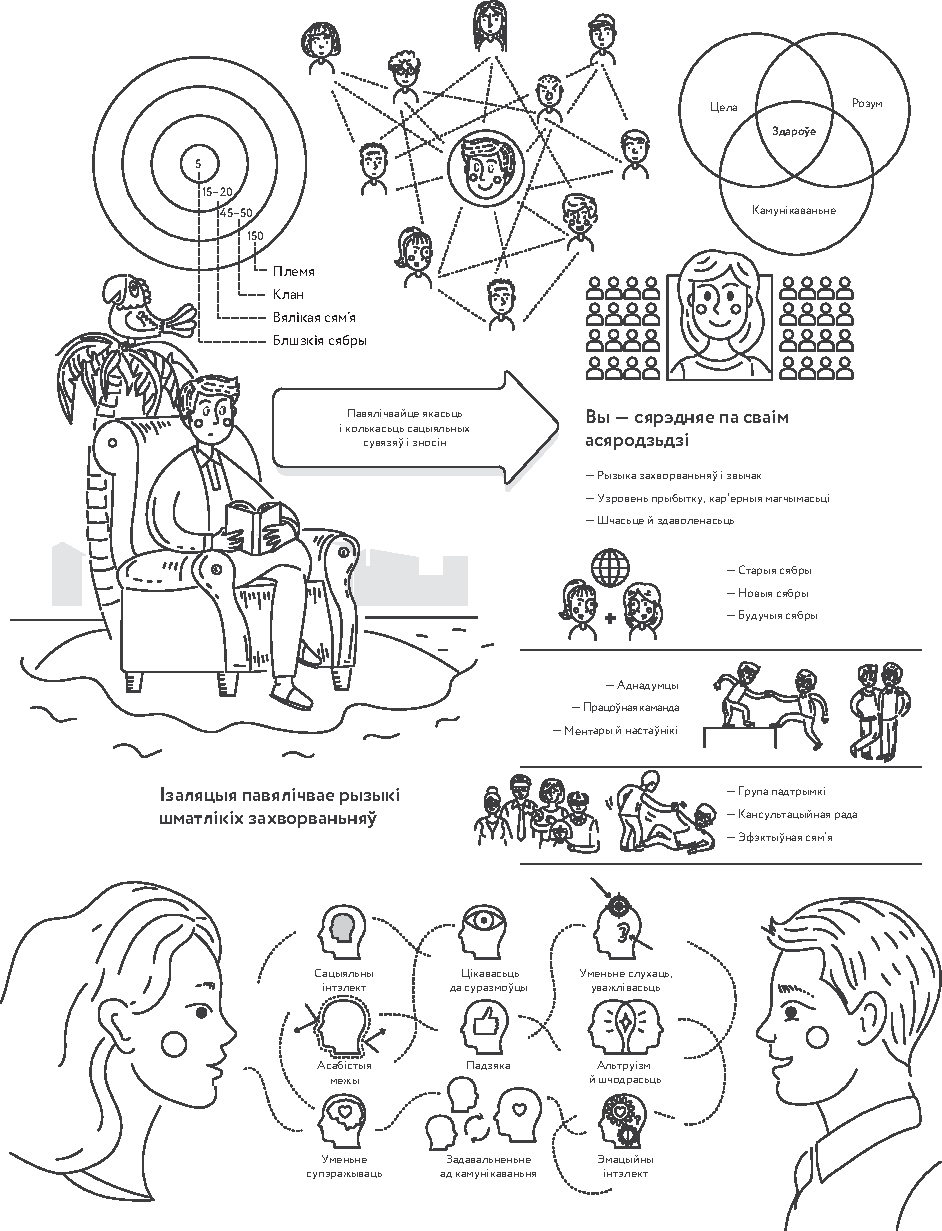
\includegraphics[width=\textwidth]{willpower/ch10/full.pdf}  
\end{figure*}
